%*****************************************
\chapter{Preliminary Results}
\label{chapter:chapter results}
%*****************************************

In this chapter, we explore the latest findings and ongoing research that form a crucial part of my PhD work. These results bear significant relevance to this thesis and enrich our understanding of the research domain, although still in progress and yet to be formally published. By including these preliminary findings, we aim to provide a comprehensive and up-to-date exploration of the topic. It is important to note that these findings are presented as drafts and are subject to further refinement and validation before publication.

\section{Result I}

\textbf{Social network influences on obesity in a general youth population.}

In recent years studies have evaluated the effect of peer pressure on obesity, via close friend networks in adults \cite{Christakis2007, Oliveira2013, Powell2015} and adolescents \cite{Fowler2008}, or direct advertising of junk food \cite{Dixon2007} or healthy habits \cite{Turner2017}. These studies have shown that people’s health, including obesity, tends to become similar to those in their social network. We would like to check if these results also apply to our student population and how these evolve over time.

In these results (tables \ref{table:resultOneBigTable}, \ref{table:resultSimulations}  figures \ref{figure:Results1general}, \ref{figure:Results1evolutionBMI}), first, we showed the social dynamics with respect to BMI (table \ref{table:resultOneBigTable}). We show that this population behaves similarly to other student populations \cite{DIXON20071311, Deoke2012, Lasserre2007}, and there is a bias in forming friendships with respect to BMI. "Overweight" and "Obese" students tend to form connections with each other, while at the same "Obese" students have lower connectivity are more isolated in the network, and seem to have a negative bias towards "Healthy" students. On the other hand, "Healthy" form connections mostly among themselves, with a negative bias toward both "Overweight" and "Obese". Using the same simulation technique as in Paper A (section \ref{sec:MetodologySimulations}), we also show a bias toward obesity spread in all networks (table \ref{table:resultSimulations}), being stronger in the "Sports" network, and weaker in the "School" network.

    \begin{table}

    \caption{ Bias with respect to the total number of relationships between each BMI category. The top column shows the absolute and relative frequencies of the population (n = 1034). People with unknown BMI are excluded from the analysis (n = 4). Each combination of categories represents people who nominate a friend (rows) and people who are nominated (columns). Each cell is divided into three parts, the left-most is the total number of relationships in this combination, the center one is the expected number of relationships (only given if a bias was found), the right part contains an arrow indicating over (up \textcolor{Green}{\textbf{↑}}) or underrepresented (down \textcolor{Red}{\textbf{↓}}) using a two-sided binomial test with at least p-value < 0.1.  The table Xi² test is < $10^{-10}$. In the bottom and to the left, we have the marginal absolute and relative frequencies for each combination. }

    \centering

    \label{table:resultOneBigTable}

    \renewcommand{\arraystretch}{1.2}

    \scalebox{0.70}{

    \begin{tabular}{|l|rrr:rrc:rrc:rrc|rr|} 
    
    \hline
    
    \begin{tabular}[c]{@{}l@{}}\end{tabular} &
    \multicolumn{3}{c}{{\cellcolor[rgb]{0.937,0.937,0.937}}
    
    \begin{tabular}[c]{@{}>{\cellcolor[rgb]{0.937,0.937,0.937}}c@{}}Underweight \\ n = 110 , f = .106\end{tabular}} &
    \multicolumn{3}{c}{{\cellcolor[rgb]{0.937,0.937,0.937}}
    
    \begin{tabular}[c]{@{}>{\cellcolor[rgb]{0.937,0.937,0.937}}c@{}}Healthy \\ n = 710 , f = .684\end{tabular}} &
    \multicolumn{3}{c}{{\cellcolor[rgb]{0.937,0.937,0.937}}
    
    \begin{tabular}[c]{@{}>{\cellcolor[rgb]{0.937,0.937,0.937}}c@{}}Overweight \\ n = 147 , f = .142\end{tabular}} &
    \multicolumn{3}{c|}{{\cellcolor[rgb]{0.937,0.937,0.937}}
    
    \begin{tabular}[c]{@{}>{\cellcolor[rgb]{0.937,0.937,0.937}}c@{}}Obese \\ n = 67 , f = .064\end{tabular}} &
    
    \multicolumn{1}{c}{{\cellcolor[rgb]{0.886,0.937,0.851}}Total} & \multicolumn{1}{c|}{{\cellcolor[rgb]{0.886,0.937,0.851}}Freq}  \\ 
    
    \hline
    
    {\cellcolor[rgb]{0.937,0.937,0.937}}Underweight & 47  &  & & 285  & & \multicolumn{1}{r:}{} & 48  & & \multicolumn{1}{r:}{} & 24 & & \multicolumn{1}{r|}{} & 404 & 10.8\% \\
    
    {\cellcolor[rgb]{0.937,0.937,0.937}}Healthy                                             & 282 &  &                                                                                                                                                               & 1870 & (1822) & \textbf{\textcolor[rgb]{0,0.502,0}{↑}}                                                                                                                      & 345 & (367) & \textbf{\textcolor{red}{↓}}                                                                                                                             & 90 & (122) & \textcolor{red}{↓}                                                                                                                                  & 2587                                                          & 69.1\%                                                         \\
{\cellcolor[rgb]{0.937,0.937,0.937}}Overweight                                          & 46  &  &                                                                                                                                                               & 347  &        &                                                                                                                                                    & 97  & (74)  & \textbf{\textcolor[rgb]{0,0.502,0}{↑}}                                                                                                                  & 34 & (24)  & \textcolor[rgb]{0,0.502,0}{\textbf{↑}}                                                                                                                       & 524                                                           & 14.0\%                                                         \\
{\cellcolor[rgb]{0.937,0.937,0.937}}Obese                                               & 22  &  &                                                                                                                                                               & 135  & (160)  & \textcolor{red}{\textbf{↓}}                                                                                                                                 & 42  & (32)  & \textcolor[rgb]{0,0.502,0}{\textbf{↑}}                                                                                                                  & 29 & (10)  & \textbf{\textcolor[rgb]{0,0.502,0}{↑}}                                                                                                                       & 228                                                           & 6.1\%                                                          \\ 
\hline
{\cellcolor[rgb]{0.886,0.937,0.851}}Total                                               & \multicolumn{3}{c}{397}                                                                                                                                                & \multicolumn{3}{c}{2637}                                                                                                                                           & \multicolumn{3}{c}{532}                                                                                                                                               & \multicolumn{3}{c|}{177}                                                                                                                                         & \multicolumn{1}{l}{3743}                                      & \multicolumn{1}{l|}{}                                          \\
{\cellcolor[rgb]{0.886,0.937,0.851}}Frequency                                           & \multicolumn{3}{c}{10.6\%}                                                                                                                                             & \multicolumn{3}{c}{70.5\%}                                                                                                                                         & \multicolumn{3}{c}{14.2\%}                                                                                                                                            & \multicolumn{3}{c|}{4.7\%}                                                                                                                                       & \multicolumn{1}{l}{}                                          & \multicolumn{1}{l|}{100\%}                                     \\
\hline
\end{tabular}

}



\end{table}



\begin{table}[H]

\caption{Results of the spread of BMI across all networks simulations. The first column is the name of the network. Second is how many relationships are in that network. The third column is how many of those relationships share the same BMI category. The next 7 columns are the details of the simulation results, with the important one being the ”Average“ and ”SD (Standard Deviation)”, which shows how many same-to-same relationships in average we had in the 1000 simulations, using a network with the same topology but randomizing the BMI according to the BMI probability density data of the original network. The last column is the p-value, rounded to 3 decimals, which shows if there is a significant difference between the averaged same-to-same simulated relationship and the real same-to-same relationships.}

\centering

\label{table:resultSimulations}

\renewcommand{\arraystretch}{1.2}
\scalebox{0.70}{

\begin{tabular}{l|rr|rrrrrrr|r}
\cline{2-10}
                                                      & \multicolumn{2}{c|}{\cellcolor[HTML]{F7CAAC}Real networks}                                                                         & \multicolumn{7}{c|}{\cellcolor[HTML]{FFE599}Simulated 1000 networks}                                                                                                                                                                                                                                                                                             & \multicolumn{1}{c}{}                                 \\ \hline
\rowcolor[HTML]{FFF2CC} 
\multicolumn{1}{|c|}{\cellcolor[HTML]{D9E2F3}Network} & \multicolumn{1}{c}{\cellcolor[HTML]{FBE4D5}Total Relationships} & \multicolumn{1}{c|}{\cellcolor[HTML]{FBE4D5}Equal Relationships} & \multicolumn{1}{c}{\cellcolor[HTML]{FFF2CC}MIN} & \multicolumn{1}{c}{\cellcolor[HTML]{FFF2CC}Q1} & \multicolumn{1}{c}{\cellcolor[HTML]{FFF2CC}Median} & \multicolumn{1}{c}{\cellcolor[HTML]{FFF2CC}Average} & \multicolumn{1}{c}{\cellcolor[HTML]{FFF2CC}Q3} & \multicolumn{1}{c}{\cellcolor[HTML]{FFF2CC}MAX} & \multicolumn{1}{c|}{\cellcolor[HTML]{FFF2CC}SD} & \multicolumn{1}{c|}{\cellcolor[HTML]{E2EFD9}P-value} \\ \hline
\multicolumn{1}{|l|}{Overall}                         & {\color[HTML]{9B9B9B} 3767}                                     & 2043                                                             & {\color[HTML]{9B9B9B} 1761}                     & {\color[HTML]{9B9B9B} 1853}                    & {\color[HTML]{9B9B9B} 1893}                        & 1894.1                                              & {\color[HTML]{9B9B9B} 1934}                    & {\color[HTML]{9B9B9B} 2077}                     & {\color[HTML]{9B9B9B} 59.5}                     & \multicolumn{1}{r|}{0.006}                           \\
\multicolumn{1}{|l|}{Physical}                        & {\color[HTML]{9B9B9B} 2823}                                     & 1584                                                             & {\color[HTML]{9B9B9B} 1233}                     & {\color[HTML]{9B9B9B} 1368}                    & {\color[HTML]{9B9B9B} 1402}                        & 1406.1                                              & {\color[HTML]{9B9B9B} 1445}                    & {\color[HTML]{9B9B9B} 1561}                     & {\color[HTML]{9B9B9B} 59.6}                     & \multicolumn{1}{r|}{0.001}                           \\
\multicolumn{1}{|l|}{School}                          & {\color[HTML]{9B9B9B} 2979}                                     & 1590                                                             & {\color[HTML]{9B9B9B} 1337}                     & {\color[HTML]{9B9B9B} 1459}                    & {\color[HTML]{9B9B9B} 1490}                        & 1493.7                                              & {\color[HTML]{9B9B9B} 1536}                    & {\color[HTML]{9B9B9B} 1647}                     & {\color[HTML]{9B9B9B} 59.9}                     & \multicolumn{1}{r|}{0.054}                           \\
\multicolumn{1}{|l|}{Sports}                          & {\color[HTML]{9B9B9B} 598}                                      & 415                                                              & {\color[HTML]{9B9B9B} 257}                      & {\color[HTML]{9B9B9B} 289}                     & {\color[HTML]{9B9B9B} 303}                         & 301.9                                               & {\color[HTML]{9B9B9B} 314}                     & {\color[HTML]{9B9B9B} 355}                      & {\color[HTML]{9B9B9B} 19.1}                     & \multicolumn{1}{r|}{\textless{}0.0001}               \\
\multicolumn{1}{|l|}{Home}                            & {\color[HTML]{9B9B9B} 1247}                                     & 722                                                              & {\color[HTML]{9B9B9B} 563}                      & {\color[HTML]{9B9B9B} 603}                     & {\color[HTML]{9B9B9B} 621}                         & 624.3                                               & {\color[HTML]{9B9B9B} 645}                     & {\color[HTML]{9B9B9B} 709}                      & {\color[HTML]{9B9B9B} 29.9}                     & \multicolumn{1}{r|}{0.001}                           \\
\multicolumn{1}{|l|}{Other}                           & {\color[HTML]{9B9B9B} 1095}                                     & 612                                                              & {\color[HTML]{9B9B9B} 488}                      & {\color[HTML]{9B9B9B} 532}                     & {\color[HTML]{9B9B9B} 552}                         & 552.7                                               & {\color[HTML]{9B9B9B} 575}                     & {\color[HTML]{9B9B9B} 623}                      & {\color[HTML]{9B9B9B} 28.8}                     & \multicolumn{1}{r|}{0.020}                           \\ \hline
\end{tabular}

}



\end{table}

We checked for the general evolution of BMI over time (figure \ref{figure:Results1general}). We observed that roughly half of the “Underweights” go into the “Healthy” group while almost none of the “Healthy” descent into the “Underweights”. However, a similar trend is seen with a big group of “Healthy” going into “Overweight” without barely “Overweight” descending into “Healthy”. There is also another group going from “Overweight” to “Obese”; this group is larger than the group descending to “Healthy”. Both “Underweight” and “Healthy” groups decrease in size while both “Overweight” and “Obese” increase. Some from the “Obese” group descent into the “Overweight” group, but not enough to compensate for those new students entering the group. The average BMI (kg/m2) in FF1 was 22.57 ± 4.23, and in FF2 was 23.32 ± 4.25. For men, in FF1 was 22.51 ± 4.22 and 23.55 ± 4.19 in FF2. For women was 22.62 ± 4.24 in FF1 and 23.12 ± 4.30 in FF2.

    \begin{figure}[ht]
        \centering
            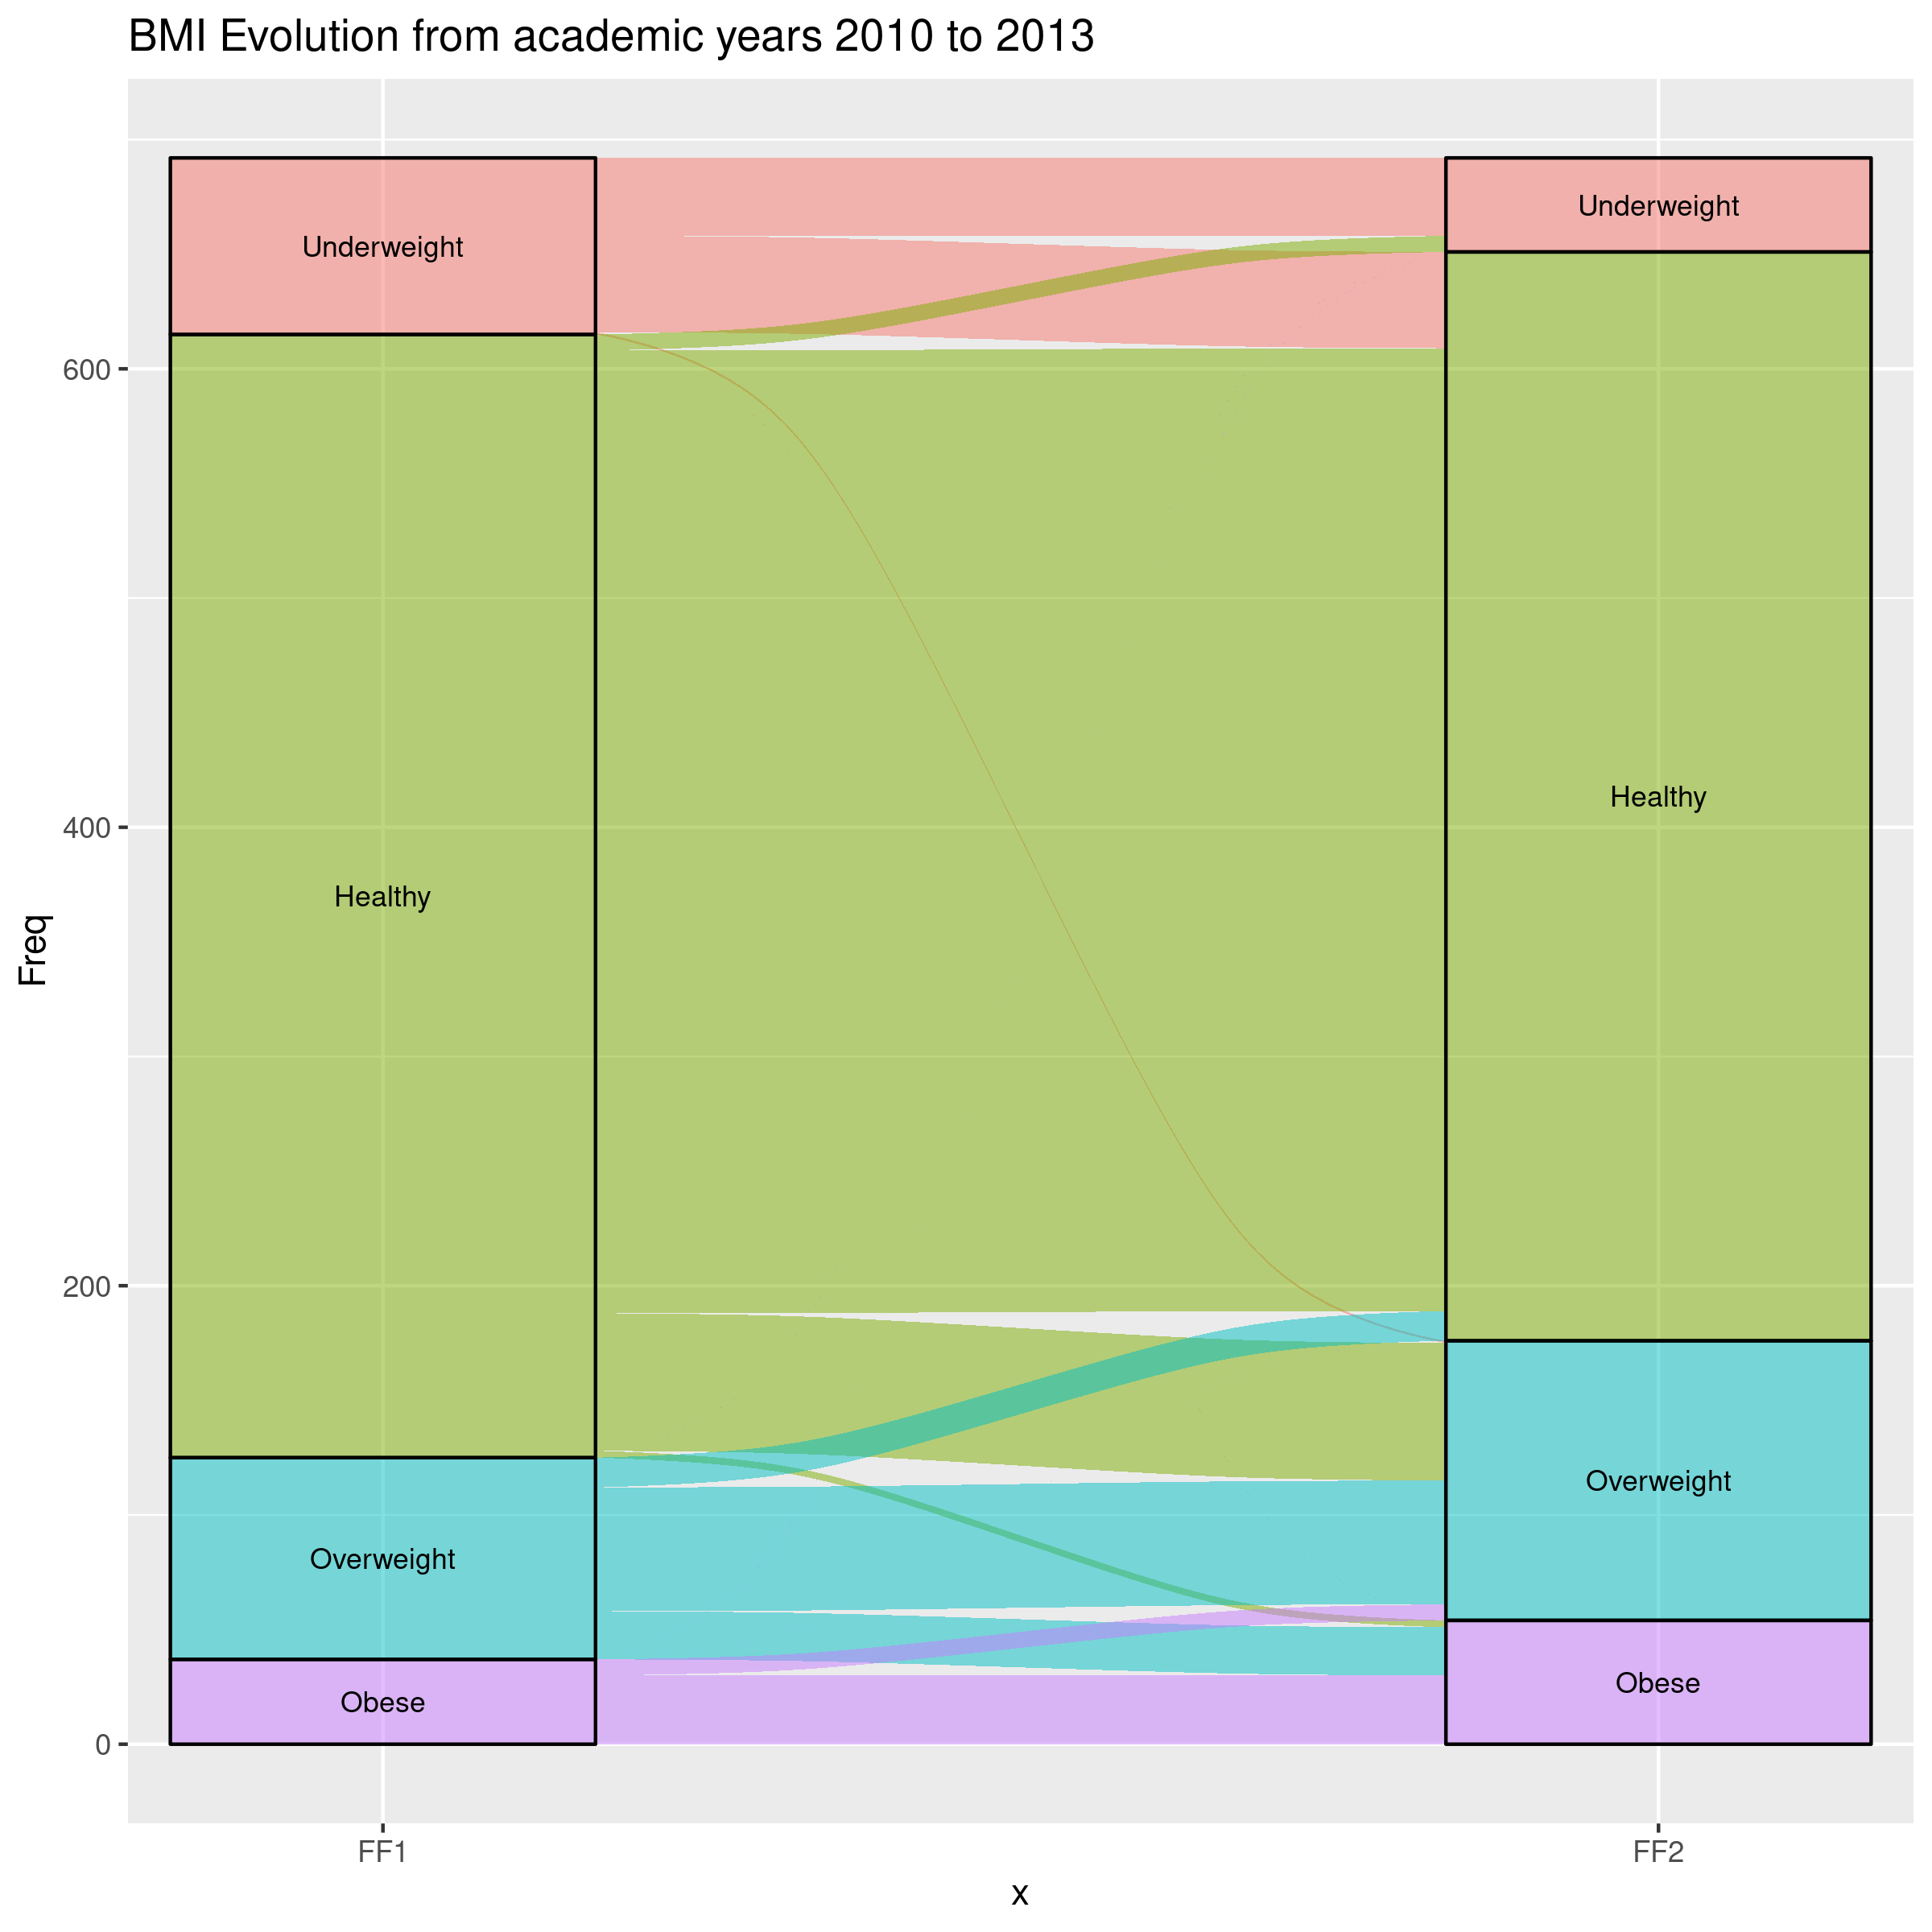
\includegraphics[width=0.75\linewidth]{figures/Results/ResultOne/generalEvolution.png } 
        \caption{An overview of the evolution of BMI from Fit Futures 1 (2010-2011) to Fit Futures 2 (2012-2013) for every student with valid BMI data in both studies (n = 692). On the left column, we have the FF1 BMI categories. In the right column, we have the FF2 categories two years later. The threads from left to right indicate the evolution of each person with respect to the BMI category.}
        \label{figure:Results1general}
    \end{figure}

We also tested if the number of high BMI friends is related to the BMI value in FF2 (figure \ref{figure:Results1evolutionBMI}). On average, the “Healthy” and “Underweight” groups tend to go down in FF2, the greater the number of friends with BMI>25 they had during FF1. We only see a sharp decrease in “Overweight” for the number of friends equal to 5, but they go into the “Obese” category instead which is a sharp increase in this group. Using logistic regression we estimated an 8.5\% increase in the risk of high BMI with respect to each additional "Overweight" or "Obese" friend. We also show that as the number of friends in FF1 with BMI > 25 increases, there is a higher probability of not landing in the "Healthy" group in FF2, and is also likely that the student will land in "Overweight" or "Obese" instead.

    \begin{figure}[ht]
        \centering
            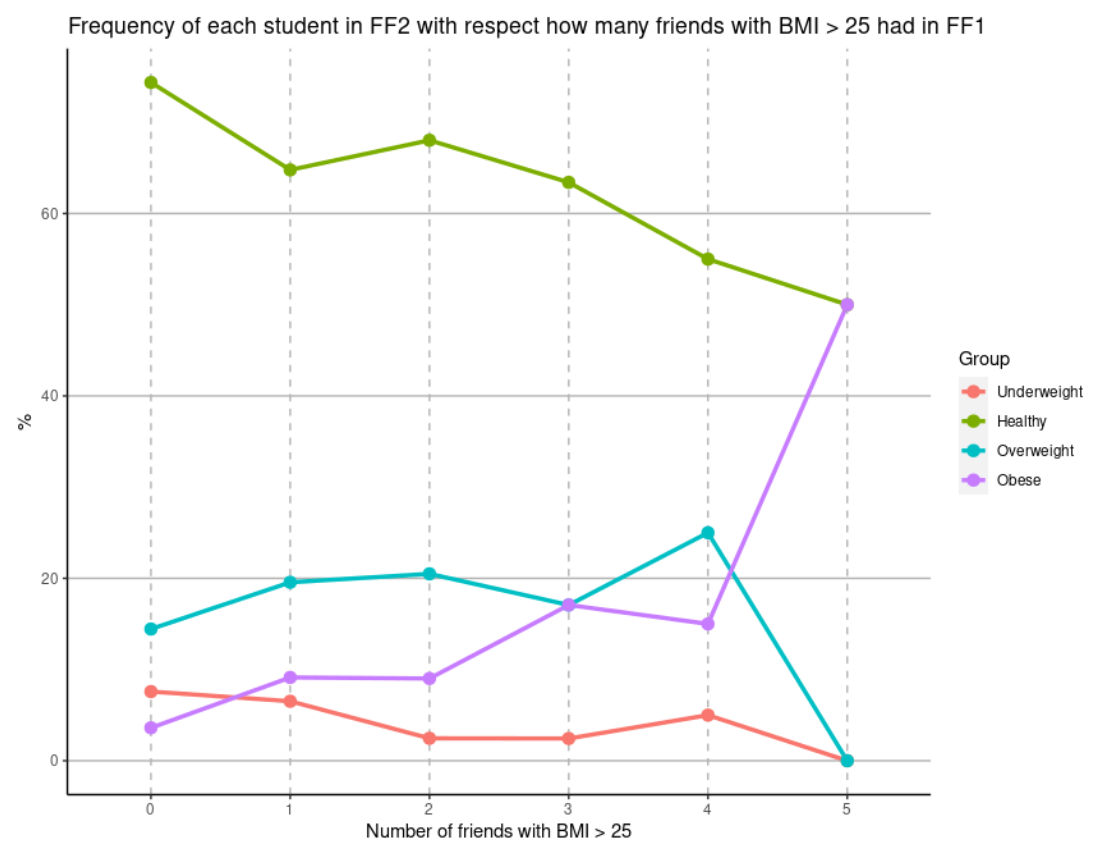
\includegraphics[width=0.75\linewidth]{figures/Results/ResultOne/bmiInfluence.png } 
        \caption{ The influence of friends from FF1 have with respect to FF2 BMI. The X-axis is the number of friends in FF1 with BMI>25 kg/m2 The Y-axis is the relative number of students belonging to each BMI category in FF2.}
        \label{figure:Results1evolutionBMI}
    \end{figure}

Overall, these results seem to indicate that friendship is stagnated and students tend to keep within the same BMI group. And more importantly, an individual with "Healthy" friends has a better chance of being "Healthy" in the future, and an individual with "Overweight" or "Obese" friends has also a better chance of being "Overweight" or "Obese" in the future as well.


\section{Result II}

\textbf{Social network influences on inflammatory response in a general youth population.}

Chronic inflammation is a health concern with evidence suggesting that it contributes to the pathogenesis of numerous diseases, including cancer, cardiovascular disease, diabetes, and neurodegenerative disorders. Obesity has been shown to be correlated from childhood to adulthood \cite{Woo2019}, while also being responsible for a range of adverse health conditions. Inflammation is shown to vary as a function of social isolation; in particular social behavior and the inflammatory process seem to be regulating one another \cite{Zhang2015, Karczewski2018, Safaei2021, Eisenberger2016, Bang2019, Henriquez2022, Koyama2021}. Obesity is also an underlying condition in both chronic inflammation and metabolic diseases \cite{Lee2013, Karczewski2018, Dhurandhar2014CounteringTE}. In this explorative study, we investigate how the three concepts of inflammation in the form of a 92 proteomic assay, obesity in the form of anthropometric variables, and social interaction in the form of our network of friends, are related to one another. In particular, we look if there is a similarity of inflammation among social contacts. We found some results in the data that suggest that inflammatory markers are common among friends of the same sex and the same high school suggesting that social influence has an underlying link.

To evaluate if there is a correlation between each person and his/her friends’ biomarker levels, we tried regression models (linear, quadratic, logarithmic, or exponential) using each person’s friends’ average biomarker level as the independent variable, and the person’s biomarker levels as the dependent variable. Without any stratification by sex or by high school, we found no statistically relevant results for any biomarker. We found no correlation for sex stratification using all high schools. But biomarker levels are influenced by sex and social influence is driven by high school. If we stratify by these two variables; we found a total of 50 biomarkers for men and 46 for women that are significant with respect to some high schools (tables \ref{table:Result1MalesRegression} and \ref{table:Result1FemalesRegression}). This suggests that some biomarker levels are influenced by the student’s social network, and in particular by high school, which has a relevant homophily coefficient (87.85\% p-value <0.0001). Furthermore, high schools where blood samples were extracted later during the academic year (March / April 2011) show a higher amount of biomarkers correlation in contrast with other schools (October 2010 to March 2011). For High School 5, we found 13 markers for men, 11 for women; for High School 6, 23 for men, 17 for women; and for the rest of high schools combined 14 for men, 18 for women.

\begin{table}[ht]

\caption{ Overview of all biomarkers with respect to each high school (n=8) for men. All biomarkers with either R2 < 0.2 and p-value > 0.05, are hidden from the tables. P-values are expressed in GP Prism 5.04/d format.}

\centering

\renewcommand{\arraystretch}{1.2}

\scalebox{0.70}{
\begin{tabular}{clll}
\rowcolor[HTML]{01C0DB} 
{\color[HTML]{FFFFFF} \textbf{Highschool}} & {\color[HTML]{FFFFFF} \textbf{Protein}}                                               & {\color[HTML]{FFFFFF} \textbf{R2}} & {\color[HTML]{FFFFFF} \textbf{P-value}} \\ \hline
                                           & C-X-C motif chemokine 9                                                               & 0.26                               & *                                       \\
                                           & Eotaxin                                                                               & 0.33                               & **                                      \\
                                           & Interleukin-10                                                                        & 0.55                               & ****                                    \\
                                           & Interleukin-10 receptor subunit alpha                                                 & 0.25                               & **                                      \\
                                           & \cellcolor[HTML]{EFEFEF}Interleukin-13                                                & \cellcolor[HTML]{EFEFEF}0.66       & \cellcolor[HTML]{EFEFEF}****            \\
                                           & \cellcolor[HTML]{EFEFEF}Interleukin-33                                                & \cellcolor[HTML]{EFEFEF}0.27       & \cellcolor[HTML]{EFEFEF}**              \\
                                           & \cellcolor[HTML]{EFEFEF}Interleukin-6                                                 & \cellcolor[HTML]{EFEFEF}0.28       & \cellcolor[HTML]{EFEFEF}*               \\
                                           & \cellcolor[HTML]{EFEFEF}Interleukin-8                                                 & \cellcolor[HTML]{EFEFEF}0.24       & \cellcolor[HTML]{EFEFEF}**              \\
                                           & Macrophage colony-stimulating factor 1                                                & 0.49                               & ****                                    \\
\multirow{-10}{*}{H2}                      & Oncostatin-M                                                                          & 0.26                               & *                                       \\ \hline
                                           & Cystatin D                                                                            & 0.21                               & **                                      \\
\multirow{-2}{*}{H3}                       & STAM-binding protein                                                                  & 0.23                               & ***                                     \\ \hline
H4                                         & \cellcolor[HTML]{EFEFEF}Leukemia inhibitory factor receptor                           & \cellcolor[HTML]{EFEFEF}0.27       & \cellcolor[HTML]{EFEFEF}***             \\ \hline
                                           & \cellcolor[HTML]{EFEFEF}Adenosine Deaminase                                           & \cellcolor[HTML]{EFEFEF}0.44       & \cellcolor[HTML]{EFEFEF}****            \\
                                           & \cellcolor[HTML]{EFEFEF}Beta-nerve growth factor                                      & \cellcolor[HTML]{EFEFEF}0.22       & \cellcolor[HTML]{EFEFEF}**              \\
                                           & \cellcolor[HTML]{EFEFEF}C-C motif chemokine 28                                        & \cellcolor[HTML]{EFEFEF}0.28       & \cellcolor[HTML]{EFEFEF}**              \\
                                           & C-X-C motif chemokine 11                                                              & 0.21                               & *                                       \\
                                           & CD40L receptor                                                                        & 0.29                               & **                                      \\
                                           & CUB domain-containing protein 1                                                       & 0.23                               & *                                       \\
                                           & Fractalkine                                                                           & 0.48                               & ***                                     \\
                                           & \cellcolor[HTML]{EFEFEF}Interleukin-10                                                & \cellcolor[HTML]{EFEFEF}0.21       & \cellcolor[HTML]{EFEFEF}**              \\
                                           & \cellcolor[HTML]{EFEFEF}Interleukin-10 receptor subunit alpha                         & \cellcolor[HTML]{EFEFEF}0.34       & \cellcolor[HTML]{EFEFEF}**              \\
                                           & \cellcolor[HTML]{EFEFEF}Interleukin-17C                                               & \cellcolor[HTML]{EFEFEF}0.24       & \cellcolor[HTML]{EFEFEF}**              \\
                                           & \cellcolor[HTML]{EFEFEF}Macrophage colony-stimulating factor 1                        & \cellcolor[HTML]{EFEFEF}0.24       & \cellcolor[HTML]{EFEFEF}*               \\
                                           & Monocyte chemotactic protein 3                                                        & 0.21                               & **                                      \\
\multirow{-13}{*}{H5}                      & Tumor necrosis factor receptor superfamily member 9                                   & 0.4                                & ***                                     \\ \hline
                                           & Artemin                                                                               & 0.32                               & *                                       \\
                                           & Beta-nerve growth factor                                                              & 0.27                               & *                                       \\
                                           & \cellcolor[HTML]{EFEFEF}C-C motif chemokine 20                                        & \cellcolor[HTML]{EFEFEF}0.57       & \cellcolor[HTML]{EFEFEF}**              \\
                                           & \cellcolor[HTML]{EFEFEF}C-C motif chemokine 25                                        & \cellcolor[HTML]{EFEFEF}0.45       & \cellcolor[HTML]{EFEFEF}**              \\
                                           & \cellcolor[HTML]{EFEFEF}C-C motif chemokine 28                                        & \cellcolor[HTML]{EFEFEF}0.62       & \cellcolor[HTML]{EFEFEF}***             \\
                                           & \cellcolor[HTML]{EFEFEF}C-X-C motif chemokine 5                                       & \cellcolor[HTML]{EFEFEF}0.32       & \cellcolor[HTML]{EFEFEF}*               \\
                                           & C-X-C motif chemokine 6                                                               & 0.4                                & *                                       \\
                                           & Caspase-8                                                                             & 0.49                               & **                                      \\
                                           & CD40L receptor                                                                        & 0.72                               & ***                                     \\
                                           & CUB domain-containing protein 1                                                       & 0.63                               & ***                                     \\
                                           & \cellcolor[HTML]{EFEFEF}Delta and Notch-like epidermal growth factor-related receptor & \cellcolor[HTML]{EFEFEF}0.56       & \cellcolor[HTML]{EFEFEF}**              \\
                                           & \cellcolor[HTML]{EFEFEF}Fibroblast growth factor 23                                   & \cellcolor[HTML]{EFEFEF}0.49       & \cellcolor[HTML]{EFEFEF}**              \\
                                           & \cellcolor[HTML]{EFEFEF}Fractalkine                                                   & \cellcolor[HTML]{EFEFEF}0.41       & \cellcolor[HTML]{EFEFEF}*               \\
                                           & \cellcolor[HTML]{EFEFEF}Interferon gamma                                              & \cellcolor[HTML]{EFEFEF}0.4        & \cellcolor[HTML]{EFEFEF}*               \\
                                           & Interleukin-33                                                                        & 0.28                               & *                                       \\
                                           & Interleukin-8                                                                         & 0.57                               & **                                      \\
                                           & Leukemia inhibitory factor receptor                                                   & 0.49                               & **                                      \\
                                           & Neurotrophin-3                                                                        & 0.51                               & **                                      \\
                                           & \cellcolor[HTML]{EFEFEF}Oncostatin-M                                                  & \cellcolor[HTML]{EFEFEF}0.28       & \cellcolor[HTML]{EFEFEF}*               \\
                                           & \cellcolor[HTML]{EFEFEF}Osteoprotegerin                                               & \cellcolor[HTML]{EFEFEF}0.53       & \cellcolor[HTML]{EFEFEF}**              \\
                                           & \cellcolor[HTML]{EFEFEF}Programmed cell death 1 ligand 1                              & \cellcolor[HTML]{EFEFEF}0.47       & \cellcolor[HTML]{EFEFEF}**              \\
                                           & \cellcolor[HTML]{EFEFEF}TNF-related apoptosis-inducing ligand                         & \cellcolor[HTML]{EFEFEF}0.48       & \cellcolor[HTML]{EFEFEF}**              \\
\multirow{-23}{*}{H6}                      & Urokinase-type plasminogen activator                                                  & 0.65                               & ***                                    
\end{tabular}
}

\label{table:Result1MalesRegression}
\end{table}


\begin{table}[ht]
\caption{ Overview of all biomarkers with respect to each high school (n=8) for women. All biomarkers with either R2 < 0.2 and p-value > 0.05, are hidden from the tables. P-values are expressed in GP Prism 5.04/d format.}
\centering
\renewcommand{\arraystretch}{1.2}

\scalebox{0.70}{
\begin{tabular}{clll}
\rowcolor[HTML]{EF35AE} 
{\color[HTML]{FFFFFF} \textbf{Highschool}} & {\color[HTML]{FFFFFF} \textbf{Protein}}                                     & {\color[HTML]{FFFFFF} \textbf{R2}} & {\color[HTML]{FFFFFF} \textbf{P-value}} \\ \hline
                                           & Glial cell line-derived neurotrophic factor                                 & 0.26                               & ****                                    \\
\multirow{-2}{*}{H1}                       & Interferon gamma                                                            & 0.24                               & ***                                     \\ \hline
H2                                         & Tumor necrosis factor                                                       & 0.4                                & ****                                    \\ \hline
                                           & Fibroblast growth factor 19                                                 & 0.23                               & **                                      \\
                                           & \cellcolor[HTML]{EFEFEF}Interleukin-10 receptor subunit beta                & \cellcolor[HTML]{EFEFEF}0.25       & \cellcolor[HTML]{EFEFEF}*               \\
                                           & \cellcolor[HTML]{EFEFEF}Interleukin-33                                      & \cellcolor[HTML]{EFEFEF}0.29       & \cellcolor[HTML]{EFEFEF}**              \\
                                           & \cellcolor[HTML]{EFEFEF}Matrix metalloproteinase-10                         & \cellcolor[HTML]{EFEFEF}0.24       & \cellcolor[HTML]{EFEFEF}**              \\
                                           & \cellcolor[HTML]{EFEFEF}Neurturin                                           & \cellcolor[HTML]{EFEFEF}0.31       & \cellcolor[HTML]{EFEFEF}***             \\
                                           & Programmed cell death 1 ligand 1                                            & 0.32                               & **                                      \\
                                           & STAM-binding protein                                                        & 0.24                               & **                                      \\
                                           & Sulfotransferase 1A1                                                        & 0.22                               & *                                       \\
\multirow{-9}{*}{H4}                       & Urokinase-type plasminogen activator                                        & 0.28                               & **                                      \\ \hline
                                           & \cellcolor[HTML]{EFEFEF}C-C motif chemokine 28                              & \cellcolor[HTML]{EFEFEF}0.27       & \cellcolor[HTML]{EFEFEF}**              \\
                                           & \cellcolor[HTML]{EFEFEF}C-X-C motif chemokine 5                             & \cellcolor[HTML]{EFEFEF}0.31       & \cellcolor[HTML]{EFEFEF}**              \\
                                           & \cellcolor[HTML]{EFEFEF}C-X-C motif chemokine 9                             & \cellcolor[HTML]{EFEFEF}0.21       & \cellcolor[HTML]{EFEFEF}*               \\
                                           & \cellcolor[HTML]{EFEFEF}Interleukin-10 receptor subunit beta                & \cellcolor[HTML]{EFEFEF}0.27       & \cellcolor[HTML]{EFEFEF}***             \\
                                           & Interleukin-6                                                               & 0.32                               & ***                                     \\
                                           & Interleukin-7                                                               & 0.22                               & **                                      \\
                                           & Latency-associated peptide transforming growth factor beta-1                & 0.26                               & ***                                     \\
                                           & Matrix metalloproteinase-10                                                 & 0.22                               & **                                      \\
                                           & \cellcolor[HTML]{EFEFEF}TNF-related activation-induced cytokine             & \cellcolor[HTML]{EFEFEF}0.24       & \cellcolor[HTML]{EFEFEF}**              \\
                                           & \cellcolor[HTML]{EFEFEF}Tumor necrosis factor                               & \cellcolor[HTML]{EFEFEF}0.36       & \cellcolor[HTML]{EFEFEF}****            \\
\multirow{-11}{*}{H5}                      & \cellcolor[HTML]{EFEFEF}Vascular endothelial growth factor A                & \cellcolor[HTML]{EFEFEF}0.24       & \cellcolor[HTML]{EFEFEF}**              \\ \hline
                                           & \cellcolor[HTML]{EFEFEF}Brain-derived neurotrophic factor                   & \cellcolor[HTML]{EFEFEF}0.76       & \cellcolor[HTML]{EFEFEF}**              \\
                                           & C-C motif chemokine 23                                                      & 0.95                               & ***                                     \\
                                           & Delta and Notch-like epidermal growth factor-related receptor               & 0.85                               & ***                                     \\
                                           & Fibroblast growth factor 21                                                 & 0.66                               & **                                      \\
                                           & Fms-related tyrosine kinase 3 ligand                                        & 0.76                               & *                                       \\
                                           & \cellcolor[HTML]{EFEFEF}Interleukin-10 receptor subunit alpha               & \cellcolor[HTML]{EFEFEF}0.69       & \cellcolor[HTML]{EFEFEF}**              \\
                                           & \cellcolor[HTML]{EFEFEF}Interleukin-17A                                     & \cellcolor[HTML]{EFEFEF}0.64       & \cellcolor[HTML]{EFEFEF}*               \\
                                           & \cellcolor[HTML]{EFEFEF}Interleukin-2 receptor subunit beta                 & \cellcolor[HTML]{EFEFEF}0.75       & \cellcolor[HTML]{EFEFEF}*               \\
                                           & \cellcolor[HTML]{EFEFEF}Interleukin-20 receptor subunit alpha               & \cellcolor[HTML]{EFEFEF}0.73       & \cellcolor[HTML]{EFEFEF}**              \\
                                           & Interleukin-33                                                              & 0.64                               & **                                      \\
                                           & Interleukin-6                                                               & 0.9                                & ***                                     \\
                                           & Leukemia inhibitory factor receptor                                         & 0.89                               & ***                                     \\
                                           & Monocyte chemotactic protein 3                                              & 0.78                               & **                                      \\
                                           & \cellcolor[HTML]{EFEFEF}Neurturin                                           & \cellcolor[HTML]{EFEFEF}0.45       & \cellcolor[HTML]{EFEFEF}*               \\
                                           & \cellcolor[HTML]{EFEFEF}Osteoprotegerin                                     & \cellcolor[HTML]{EFEFEF}0.59       & \cellcolor[HTML]{EFEFEF}*               \\
                                           & \cellcolor[HTML]{EFEFEF}Stem cell factor                                    & \cellcolor[HTML]{EFEFEF}0.67       & \cellcolor[HTML]{EFEFEF}**              \\
\multirow{-17}{*}{H6}                      & \cellcolor[HTML]{EFEFEF}T cell surface glycoprotein CD6 isoform             & \cellcolor[HTML]{EFEFEF}0.45       & \cellcolor[HTML]{EFEFEF}*               \\ \hline
                                           & C-C motif chemokine 4                                                       & 0.27                               & ***                                     \\
                                           & Caspase-8                                                                   & 0.47                               & ****                                    \\
                                           & Interleukin-17C                                                             & 0.21                               & **                                      \\
                                           & Interleukin-24                                                              & 0.36                               & ****                                    \\
                                           & \cellcolor[HTML]{EFEFEF}Osteoprotegerin                                     & \cellcolor[HTML]{EFEFEF}0.21       & \cellcolor[HTML]{EFEFEF}**              \\
\multirow{-6}{*}{H8}                       & \cellcolor[HTML]{EFEFEF}Tumor necrosis factor receptor superfamily member 9 & \cellcolor[HTML]{EFEFEF}0.29       & \cellcolor[HTML]{EFEFEF}***            
\end{tabular}
}

\label{table:Result1FemalesRegression}

\end{table}

We wanted to check not only that biomarkers are similar among friends, but also different from non-friends. We defined biomarker distance as the ratio of the average square difference between each person’s biomarker level and levels among students who are not his/her friends, and the average square difference between each person’s biomarker level and levels among students who are his/her friends. We analyzed using same-sex friends, only for people with at least two friends of the same sex with valid biomarker levels. Values closer to 1 indicate no difference between each person’s friends and non-friends biomarker level average. Values greater than 1 indicate that the distance to the friends’ biomarkers is shorter (more similar) than to the non-friends biomarkers. Values smaller than 1 indicate that non-friends are closer and more similar than friends. We arbitrarily defined distances ±0.1 from 1 as relevant. We found for both men and women 14 proteins in each group with a ratio higher than 1.1, for men we found three proteins lower than 0.9, and for women, we found five proteins lower than 0.9 (tables \ref{table:Result1Friends1}, \ref{table:Result1Friends2}, \ref{table:Result1Friends3}, \ref{table:Result1Friends4}). 

\begin{table}[ht]
\caption{Ratio of average square distances between each person's biomarker level and friend's biomarker levels, and average square distance between each person's biomarker levels and non-friends biomarker levels. Values greater than 1 suggest that clusters of friends have similar biomarkers levels in comparison with the rest of the non-friend population. Relevant values are highlighted in bold, with green for >1.1 and red for <0.9. Values are rounded to two decimals but highlighted according to the original values. (Table 1 of 4)}
\centering
\renewcommand{\arraystretch}{1.2}
\begin{tabular}{lll}
\rowcolor[HTML]{FFFFC7} 
\textbf{Protein}                                        & \textbf{Men}                         & \textbf{Women}                       \\
Adenosine Deaminase                                     & {\color[HTML]{009901} \textbf{1.12}} & {\color[HTML]{C0C0C0} 1.03}          \\
Artemin                                                 & {\color[HTML]{C0C0C0} 0.98}          & {\color[HTML]{C0C0C0} 1.04}          \\
Axin-1                                                  & {\color[HTML]{C0C0C0} 1.06}          & {\color[HTML]{C0C0C0} 1.02}          \\
Brain-derived neurotrophic factor                       & {\color[HTML]{C0C0C0} 1.06}          & {\color[HTML]{009901} \textbf{1.14}} \\
\rowcolor[HTML]{EFEFEF} 
Beta-nerve growth factor                                & {\color[HTML]{009901} \textbf{1.29}} & {\color[HTML]{C0C0C0} 0.91}          \\
\rowcolor[HTML]{EFEFEF} 
Caspase-8                                               & {\color[HTML]{C0C0C0} 1.01}          & {\color[HTML]{C0C0C0} 1.04}          \\
\rowcolor[HTML]{EFEFEF} 
Eotaxin                                                 & {\color[HTML]{C0C0C0} 0.94}          & {\color[HTML]{C0C0C0} 1.04}          \\
\rowcolor[HTML]{EFEFEF} 
C-C motif chemokine 19                                  & {\color[HTML]{C0C0C0} 1}             & {\color[HTML]{C0C0C0} 0.96}          \\
C-C motif chemokine 20                                  & {\color[HTML]{C0C0C0} 1.09}          & {\color[HTML]{C0C0C0} 0.97}          \\
C-C motif chemokine 23                                  & {\color[HTML]{C0C0C0} 1.06}          & {\color[HTML]{009901} \textbf{1.1}}  \\
C-C motif chemokine 25                                  & {\color[HTML]{C0C0C0} 1.04}          & {\color[HTML]{C0C0C0} 1.02}          \\
C-C motif chemokine 28                                  & {\color[HTML]{CB0000} \textbf{0.76}} & {\color[HTML]{CB0000} \textbf{0.84}} \\
\rowcolor[HTML]{EFEFEF} 
{\color[HTML]{000000} C-C motif chemokine 3}            & {\color[HTML]{C0C0C0} 1}             & {\color[HTML]{C0C0C0} 0.96}          \\
\rowcolor[HTML]{EFEFEF} 
{\color[HTML]{000000} C-C motif chemokine 4}            & {\color[HTML]{C0C0C0} 0.98}          & {\color[HTML]{C0C0C0} 1.02}          \\
\rowcolor[HTML]{EFEFEF} 
{\color[HTML]{000000} Natural killer cell receptor 2B4} & {\color[HTML]{C0C0C0} 1.02}          & {\color[HTML]{C0C0C0} 1}             \\
\rowcolor[HTML]{EFEFEF} 
{\color[HTML]{000000} CD40L receptor}                   & {\color[HTML]{C0C0C0} 1.03}          & {\color[HTML]{C0C0C0} 1.04}          \\
T-cell surface glycoprotein CD5                         & {\color[HTML]{C0C0C0} 1.09}          & {\color[HTML]{C0C0C0} 1.07}          \\
T cell surface glycoprotein CD6 isoform                 & {\color[HTML]{C0C0C0} 1.04}          & {\color[HTML]{C0C0C0} 0.97}          \\
CUB domain-containing protein 1                         & {\color[HTML]{C0C0C0} 1.04}          & {\color[HTML]{009901} \textbf{1.14}} \\
Macrophage colony-stimulating factor 1                  & {\color[HTML]{C0C0C0} 1.01}          & {\color[HTML]{009901} \textbf{1.13}} \\
\rowcolor[HTML]{EFEFEF} 
Cystatin D                                              & {\color[HTML]{C0C0C0} 1.04}          & {\color[HTML]{C0C0C0} 0.97}          \\
\rowcolor[HTML]{EFEFEF} 
Fractalkine                                             & {\color[HTML]{009901} \textbf{1.12}} & {\color[HTML]{C0C0C0} 1.03}          \\
\rowcolor[HTML]{EFEFEF} 
C-X-C motif chemokine 1                                 & {\color[HTML]{C0C0C0} 1.07}          & {\color[HTML]{C0C0C0} 1.08}          \\
\rowcolor[HTML]{EFEFEF} 
C-X-C motif chemokine 10                                & {\color[HTML]{C0C0C0} 1.05}          & {\color[HTML]{C0C0C0} 0.97}         
\end{tabular}

\label{table:Result1Friends1}
\end{table}


\begin{table}[ht]
\caption{Ratio of average square distances (Table 2 of 4)}
\centering
\renewcommand{\arraystretch}{1.2}
\begin{tabular}{lll}
\rowcolor[HTML]{FFFFC7} 
\textbf{Protein}                                              & \textbf{Men}                         & \textbf{Women}                       \\
C-X-C motif chemokine 11                                      & {\color[HTML]{C0C0C0} 1.05}          & {\color[HTML]{C0C0C0} 1.02}          \\
C-X-C motif chemokine 5                                       & {\color[HTML]{C0C0C0} 1.01}          & {\color[HTML]{C0C0C0} 1.09}          \\
C-X-C motif chemokine 6                                       & {\color[HTML]{C0C0C0} 0.95}          & {\color[HTML]{C0C0C0} 1}             \\
C-X-C motif chemokine 9                                       & {\color[HTML]{009901} \textbf{1.11}} & {\color[HTML]{C0C0C0} 1}             \\
\rowcolor[HTML]{EFEFEF} 
Delta and Notch-like epidermal growth factor-related receptor & {\color[HTML]{009901} \textbf{1.14}} & {\color[HTML]{C0C0C0} 1.09}          \\
\rowcolor[HTML]{EFEFEF} 
Eukaryotic translation initiation factor 4E-binding protein 1 & {\color[HTML]{009901} \textbf{1.21}} & {\color[HTML]{C0C0C0} 1.03}          \\
\rowcolor[HTML]{EFEFEF} 
Protein S100-A12                                              & {\color[HTML]{C0C0C0} 1.03}          & {\color[HTML]{C0C0C0} 0.99}          \\
\rowcolor[HTML]{EFEFEF} 
Fibroblast growth factor 19                                   & {\color[HTML]{C0C0C0} 1.08}          & {\color[HTML]{C0C0C0} 1.06}          \\
Fibroblast growth factor 21                                   & {\color[HTML]{C0C0C0} 1.07}          & {\color[HTML]{009901} \textbf{1.12}} \\
Fibroblast growth factor 23                                   & {\color[HTML]{C0C0C0} 1.08}          & {\color[HTML]{C0C0C0} 1.06}          \\
Fibroblast growth factor 5                                    & {\color[HTML]{C0C0C0} 1.03}          & {\color[HTML]{C0C0C0} 0.9}           \\
Fms-related tyrosine kinase 3 ligand                          & {\color[HTML]{009901} \textbf{1.11}} & {\color[HTML]{C0C0C0} 0.99}          \\
\rowcolor[HTML]{EFEFEF} 
Glial cell line-derived neurotrophic factor                   & {\color[HTML]{C0C0C0} 1.08}          & {\color[HTML]{C0C0C0} 1.05}          \\
\rowcolor[HTML]{EFEFEF} 
Hepatocyte growth factor                                      & {\color[HTML]{C0C0C0} 1.04}          & {\color[HTML]{C0C0C0} 1}             \\
\rowcolor[HTML]{EFEFEF} 
Interferon gamma                                              & {\color[HTML]{C0C0C0} 1.04}          & {\color[HTML]{CB0000} \textbf{0.79}} \\
\rowcolor[HTML]{EFEFEF} 
Interleukin-10                                                & {\color[HTML]{C0C0C0} 0.99}          & {\color[HTML]{009901} \textbf{1.16}} \\
Interleukin-10 receptor subunit alpha                         & {\color[HTML]{C0C0C0} 1.03}          & {\color[HTML]{C0C0C0} 0.96}          \\
Interleukin-10 receptor subunit beta                          & {\color[HTML]{009901} \textbf{1.1}}  & {\color[HTML]{C0C0C0} 1.06}          \\
Interleukin-12 subunit beta                                   & {\color[HTML]{C0C0C0} 1.08}          & {\color[HTML]{C0C0C0} 1}             \\
Interleukin-13                                                & {\color[HTML]{C0C0C0} 1.04}          & {\color[HTML]{009901} \textbf{1.11}} \\
\rowcolor[HTML]{EFEFEF} 
Interleukin-15 receptor subunit alpha                         & {\color[HTML]{C0C0C0} 1.02}          & {\color[HTML]{C0C0C0} 1}             \\
\rowcolor[HTML]{EFEFEF} 
Interleukin-17A                                               & {\color[HTML]{C0C0C0} 0.95}          & {\color[HTML]{C0C0C0} 1}             \\
\rowcolor[HTML]{EFEFEF} 
Interleukin-17C                                               & {\color[HTML]{C0C0C0} 1.06}          & {\color[HTML]{C0C0C0} 1.04}          \\
\rowcolor[HTML]{EFEFEF} 
Interleukin-18                                                & {\color[HTML]{C0C0C0} 0.97}          & {\color[HTML]{C0C0C0} 1.05}          \\
                                                              &                                      &                                      \\
                                                              &                                      &                                      \\
                                                              &                                      &                                     
\end{tabular}
\label{table:Result1Friends2}
\end{table}


\begin{table}[ht]
\caption{Ratio of average square distances (Table 3 of 4)}
\centering
\renewcommand{\arraystretch}{1.2}
\begin{tabular}{lll}
\rowcolor[HTML]{FFFFC7} 
\textbf{Protein}                        & \textbf{Men}                         & \textbf{Women}                       \\
Interleukin-18 receptor 1               & {\color[HTML]{C0C0C0} 0.94}          & {\color[HTML]{C0C0C0} 1.08}          \\
Interleukin-1 alpha                     & {\color[HTML]{C0C0C0} 1.09}          & {\color[HTML]{009901} \textbf{1.12}} \\
Interleukin-2                           & {\color[HTML]{C0C0C0} 1.09}          & {\color[HTML]{C0C0C0} 0.97}          \\
Interleukin-20                          & {\color[HTML]{009901} \textbf{1.22}} & {\color[HTML]{C0C0C0} 0.98}          \\
\rowcolor[HTML]{EFEFEF} 
Interleukin-20 receptor subunit alpha   & {\color[HTML]{C0C0C0} 1.01}          & {\color[HTML]{C0C0C0} 0.98}          \\
\rowcolor[HTML]{EFEFEF} 
Interleukin-22 receptor subunit alpha-1 & {\color[HTML]{C0C0C0} 1}             & {\color[HTML]{C0C0C0} 0.92}          \\
\rowcolor[HTML]{EFEFEF} 
Interleukin-24                          & {\color[HTML]{C0C0C0} 0.98}          & {\color[HTML]{C0C0C0} 1.03}          \\
\rowcolor[HTML]{EFEFEF} 
Interleukin-2 receptor subunit beta     & {\color[HTML]{C0C0C0} 1.05}          & {\color[HTML]{C0C0C0} 0.93}          \\
Interleukin-33                          & {\color[HTML]{C0C0C0} 1.03}          & {\color[HTML]{C0C0C0} 0.99}          \\
Interleukin-4                           & {\color[HTML]{C0C0C0} 0.98}          & {\color[HTML]{C0C0C0} 1.09}          \\
Interleukin-5                           & {\color[HTML]{CB0000} \textbf{0.87}} & {\color[HTML]{C0C0C0} 1.04}          \\
Interleukin-6                           & {\color[HTML]{C0C0C0} 0.98}          & {\color[HTML]{009901} \textbf{1.3}}  \\
\rowcolor[HTML]{EFEFEF} 
Interleukin-7                           & {\color[HTML]{C0C0C0} 1.03}          & {\color[HTML]{C0C0C0} 1}             \\
\rowcolor[HTML]{EFEFEF} 
Interleukin-8                           & {\color[HTML]{C0C0C0} 1.05}          & {\color[HTML]{C0C0C0} 1.01}          \\
\rowcolor[HTML]{EFEFEF} 
Leukemia inhibitory factor              & {\color[HTML]{C0C0C0} 0.92}          & {\color[HTML]{CB0000} \textbf{0.85}} \\
\rowcolor[HTML]{EFEFEF} 
Leukemia inhibitory factor receptor     & {\color[HTML]{C0C0C0} 1.08}          & {\color[HTML]{C0C0C0} 0.96}          \\
Monocyte chemotactic protein 1          & {\color[HTML]{C0C0C0} 1.05}          & {\color[HTML]{009901} \textbf{1.18}} \\
Monocyte chemotactic protein 2          & {\color[HTML]{C0C0C0} 0.92}          & {\color[HTML]{C0C0C0} 1.06}          \\
Monocyte chemotactic protein 3          & {\color[HTML]{C0C0C0} 1.01}          & {\color[HTML]{C0C0C0} 0.92}          \\
Monocyte chemotactic protein 4          & {\color[HTML]{C0C0C0} 1}             & {\color[HTML]{009901} \textbf{1.12}} \\
\rowcolor[HTML]{EFEFEF} 
Matrix metalloproteinase-1              & {\color[HTML]{C0C0C0} 1.05}          & {\color[HTML]{C0C0C0} 0.97}          \\
\rowcolor[HTML]{EFEFEF} 
Matrix metalloproteinase-10             & {\color[HTML]{009901} \textbf{1.11}} & {\color[HTML]{009901} \textbf{1.1}}  \\
\rowcolor[HTML]{EFEFEF} 
Neurturin                               & {\color[HTML]{C0C0C0} 0.91}          & {\color[HTML]{C0C0C0} 1.06}          \\
\rowcolor[HTML]{EFEFEF} 
Neurotrophin-3                          & {\color[HTML]{C0C0C0} 0.98}          & {\color[HTML]{C0C0C0} 1.02}         
\end{tabular}
\label{table:Result1Friends3}
\end{table}



\begin{table}[ht]
\caption{Ratio of average square distances (Table 4 of 4)}
\centering
\renewcommand{\arraystretch}{1.2}
\begin{tabular}{lll}
\rowcolor[HTML]{FFFFC7} 
\textbf{Protein}                                             & \textbf{Men}                         & \textbf{Women}                       \\
Osteoprotegerin                                              & {\color[HTML]{C0C0C0} 1.07}          & {\color[HTML]{C0C0C0} 0.98}          \\
Oncostatin-M                                                 & {\color[HTML]{C0C0C0} 1.09}          & {\color[HTML]{C0C0C0} 1.03}          \\
Programmed cell death 1 ligand 1                             & {\color[HTML]{C0C0C0} 0.93}          & {\color[HTML]{C0C0C0} 0.96}          \\
Stem cell factor                                             & {\color[HTML]{C0C0C0} 1.05}          & {\color[HTML]{C0C0C0} 1.08}          \\
\rowcolor[HTML]{EFEFEF} 
SIR2-like protein 2                                          & {\color[HTML]{C0C0C0} 1.04}          & {\color[HTML]{C0C0C0} 1.02}          \\
\rowcolor[HTML]{EFEFEF} 
Signaling lymphocytic activation molecule                    & {\color[HTML]{C0C0C0} 1.02}          & {\color[HTML]{CB0000} \textbf{0.88}} \\
\rowcolor[HTML]{EFEFEF} 
Sulfotransferase 1A1                                         & {\color[HTML]{C0C0C0} 1.01}          & {\color[HTML]{C0C0C0} 1.07}          \\
\rowcolor[HTML]{EFEFEF} 
STAM-binding protein                                         & {\color[HTML]{C0C0C0} 1.1}           & {\color[HTML]{C0C0C0} 0.99}          \\
Transforming growth factor alpha                             & {\color[HTML]{C0C0C0} 1.09}          & {\color[HTML]{C0C0C0} 1.02}          \\
Latency-associated peptide transforming growth factor beta-1 & {\color[HTML]{C0C0C0} 1.08}          & {\color[HTML]{C0C0C0} 0.99}          \\
Tumor necrosis factor                                        & {\color[HTML]{CB0000} \textbf{0.87}} & {\color[HTML]{CB0000} \textbf{0.69}} \\
TNF-beta                                                     & {\color[HTML]{C0C0C0} 1.04}          & {\color[HTML]{C0C0C0} 1.02}          \\
\rowcolor[HTML]{EFEFEF} 
Tumor necrosis factor receptor superfamily member 9          & {\color[HTML]{009901} \textbf{1.24}} & {\color[HTML]{C0C0C0} 1.08}          \\
\rowcolor[HTML]{EFEFEF} 
Tumor necrosis factor ligand superfamily member 14           & {\color[HTML]{C0C0C0} 1.08}          & {\color[HTML]{C0C0C0} 1.01}          \\
\rowcolor[HTML]{EFEFEF} 
TNF-related apoptosis-inducing ligand                        & {\color[HTML]{009901} \textbf{1.17}} & {\color[HTML]{C0C0C0} 1.01}          \\
\rowcolor[HTML]{EFEFEF} 
TNF-related activation-induced cytokine                      & {\color[HTML]{009901} \textbf{1.1}}  & {\color[HTML]{009901} \textbf{1.11}} \\
Thymic stromal lymphopoietin                                 & {\color[HTML]{C0C0C0} 1.01}          & {\color[HTML]{C0C0C0} 0.98}          \\
Tumor necrosis factor                                        & {\color[HTML]{C0C0C0} 1.02}          & {\color[HTML]{C0C0C0} 1.02}          \\
Urokinase-type plasminogen activator                         & {\color[HTML]{009901} \textbf{1.24}} & {\color[HTML]{C0C0C0} 1.08}          \\
Vascular endothelial growth factor A                         & {\color[HTML]{C0C0C0} 1}             & {\color[HTML]{009901} \textbf{1.16}}
\end{tabular}
\label{table:Result1Friends4}
\end{table}

There is also a correlation between anthropometry and inflammation (table \ref{table:BiomarkersAntropoMales} and table \ref{table:BiomarkersAntropoFemales}); Result I and Result III suggest that social contact also influences the spread of obesity which is determined by anthropometrical variables. Not all the biomarkers presented in the anthropometric variables are necessarily expressed in each high school or vice versa. Inflammation driven by obesity only, or social influence only, would have similar results in both groups, so this would hint that we have a mix of the two factors. Furthermore, we see that high schools 5 and 6 have the greatest number of biomarkers being significant compared with the rest. This seems to indicate that biomarker levels gain similarity between friends over time. We also saw that the biomarkers that were negatively correlated with respect to friends' influence do not correlate with anthropometry and very little with high schools. 

\begin{table}[ht]
\caption{Anthropometric variables with respect to biomarkers levels in men. Each cell is a p-value in GP Prism 5.04/d format. Biomarkers rows with no statistically significant p-values are hidden. All p-values are corrected for Bonferroni. }
\centering

\renewcommand{\arraystretch}{1.2}
\scalebox{0.65}{

\begin{tabular}{lcccccccc}
\rowcolor[HTML]{01C0DB} 
{\color[HTML]{FFFFFF} \textbf{Protein}}                                                                    & {\color[HTML]{FFFFFF} \textbf{Waist}} & {\color[HTML]{FFFFFF} \textbf{Hip}} & {\color[HTML]{FFFFFF} \textbf{Height}} & {\color[HTML]{FFFFFF} \textbf{Weight}} & {\color[HTML]{FFFFFF} \textbf{BMI}} & {\color[HTML]{FFFFFF} \textbf{HR}} & {\color[HTML]{FFFFFF} \textbf{SYSBP}} & {\color[HTML]{FFFFFF} \textbf{DIABP}} \\
\multicolumn{1}{l|}{C-C motif chemokine 3}                                                                 & ***                                   & **                                  & ns                                     & **                                     & **                                  & ns                                 & ns                                    & ns                                    \\
\multicolumn{1}{l|}{C-C motif chemokine 4}                                                                 & **                                    & ns                                  & ns                                     & ns                                     & ns                                  & ns                                 & ns                                    & ns                                    \\
\multicolumn{1}{l|}{CUB domain-containing protein 1}                                                       & ****                                  & ****                                & ns                                     & ****                                   & ****                                & ns                                 & ns                                    & ns                                    \\
\multicolumn{1}{l|}{Macrophage colony-stimulating factor 1}                                                & **                                    & ****                                & ns                                     & ***                                    & ***                                 & ns                                 & ns                                    & ns                                    \\
\rowcolor[HTML]{EFEFEF} 
\multicolumn{1}{l|}{\cellcolor[HTML]{EFEFEF}Delta and Notch-like epidermal growth factor-related receptor} & ns                                    & ns                                  & ns                                     & *                                      & ns                                  & ns                                 & ns                                    & ns                                    \\
\rowcolor[HTML]{EFEFEF} 
\multicolumn{1}{l|}{\cellcolor[HTML]{EFEFEF}Fibroblast growth factor 19}                                   & ns                                    & ns                                  & ns                                     & ns                                     & *                                   & ns                                 & ns                                    & ns                                    \\
\rowcolor[HTML]{EFEFEF} 
\multicolumn{1}{l|}{\cellcolor[HTML]{EFEFEF}Fibroblast growth factor 21}                                   & *                                     & ns                                  & ns                                     & ns                                     & ns                                  & ns                                 & ns                                    & ns                                    \\
\rowcolor[HTML]{EFEFEF} 
\multicolumn{1}{l|}{\cellcolor[HTML]{EFEFEF}Glial cell line-derived neurotrophic factor}                   & **                                    & ns                                  & ns                                     & *                                      & **                                  & ns                                 & ns                                    & ns                                    \\
\multicolumn{1}{l|}{Hepatocyte growth factor}                                                              & ****                                  & ***                                 & ns                                     & **                                     & ****                                & ns                                 & ns                                    & ns                                    \\
\multicolumn{1}{l|}{Interleukin-18}                                                                        & ***                                   & ***                                 & ns                                     & ***                                    & ***                                 & ns                                 & ns                                    & ns                                    \\
\multicolumn{1}{l|}{Interleukin-18 receptor 1}                                                             & ****                                  & ****                                & ns                                     & ****                                   & ****                                & ns                                 & ns                                    & ns                                    \\
\multicolumn{1}{l|}{Interleukin-6}                                                                         & ****                                  & ***                                 & ns                                     & ***                                    & ****                                & ns                                 & ns                                    & ns                                    \\
\rowcolor[HTML]{EFEFEF} 
\multicolumn{1}{l|}{\cellcolor[HTML]{EFEFEF}Monocyte chemotactic protein 3}                                & ****                                  & ****                                & ns                                     & ****                                   & ****                                & ns                                 & ns                                    & ns                                    \\
\rowcolor[HTML]{EFEFEF} 
\multicolumn{1}{l|}{\cellcolor[HTML]{EFEFEF}Stem cell factor}                                              & ****                                  & ****                                & ns                                     & ****                                   & ****                                & ns                                 & ns                                    & ns                                    \\
\rowcolor[HTML]{EFEFEF} 
\multicolumn{1}{l|}{\cellcolor[HTML]{EFEFEF}Tumor necrosis factor receptor superfamily member 9}           & ***                                   & ns                                  & ns                                     & *                                      & **                                  & ns                                 & ns                                    & ns                                   
\end{tabular}

}

\label{table:BiomarkersAntropoMales}
\end{table}


\begin{table}[ht]
\caption{Anthropometric variables with respect to biomarkers levels in women. Each cell is a p-value in GP Prism 5.04/d format. Biomarkers rows with no statistically significant p-values are hidden. All p-values are corrected for Bonferroni. }
\centering


\renewcommand{\arraystretch}{1.2}
\scalebox{0.65}{

\begin{tabular}{lcccccccc}
\rowcolor[HTML]{EF35AE} 
{\color[HTML]{FFFFFF} \textbf{Protein}}                                                                    & {\color[HTML]{FFFFFF} \textbf{Waist}} & {\color[HTML]{FFFFFF} \textbf{Hip}} & {\color[HTML]{FFFFFF} \textbf{Height}} & {\color[HTML]{FFFFFF} \textbf{Weight}} & {\color[HTML]{FFFFFF} \textbf{BMI}} & {\color[HTML]{FFFFFF} \textbf{HR}} & {\color[HTML]{FFFFFF} \textbf{SYSBP}} & {\color[HTML]{FFFFFF} \textbf{DIABP}} \\
\multicolumn{1}{l|}{Caspase-8}                                                                             & *                                     & ***                                 & ns                                     & ***                                    & **                                  & ns                                 & ns                                    & ns                                    \\
\multicolumn{1}{l|}{C-C motif chemokine 3}                                                                 & *                                     & ns                                  & ns                                     & ns                                     & ns                                  & ns                                 & ns                                    & ns                                    \\
\multicolumn{1}{l|}{CUB domain-containing protein 1}                                                       & ****                                  & ****                                & ns                                     & ****                                   & ****                                & ns                                 & ns                                    & ns                                    \\
\multicolumn{1}{l|}{Macrophage colony-stimulating factor 1}                                                & ****                                  & ***                                 & ns                                     & **                                     & **                                  & ns                                 & ns                                    & ns                                    \\
\rowcolor[HTML]{EFEFEF} 
\multicolumn{1}{l|}{\cellcolor[HTML]{EFEFEF}Delta and Notch-like epidermal growth factor-related receptor} & ns                                    & ns                                  & ns                                     & *                                      & *                                   & ns                                 & ns                                    & ns                                    \\
\rowcolor[HTML]{EFEFEF} 
\multicolumn{1}{l|}{\cellcolor[HTML]{EFEFEF}Fibroblast growth factor 21}                                   & *                                     & ns                                  & ns                                     & ns                                     & *                                   & ns                                 & ns                                    & ns                                    \\
\rowcolor[HTML]{EFEFEF} 
\multicolumn{1}{l|}{\cellcolor[HTML]{EFEFEF}Hepatocyte growth factor}                                      & ****                                  & ***                                 & ns                                     & **                                     & ***                                 & ns                                 & ns                                    & ns                                    \\
\rowcolor[HTML]{EFEFEF} 
\multicolumn{1}{l|}{\cellcolor[HTML]{EFEFEF}Interleukin-10 receptor subunit beta}                          & ****                                  & *                                   & ns                                     & **                                     & **                                  & ns                                 & ns                                    & ns                                    \\
\multicolumn{1}{l|}{Interleukin-18}                                                                        & **                                    & *                                   & ns                                     & ns                                     & **                                  & ns                                 & ns                                    & ns                                    \\
\multicolumn{1}{l|}{Interleukin-18 receptor 1}                                                             & ****                                  & ***                                 & ns                                     & ***                                    & ****                                & ns                                 & ns                                    & ns                                    \\
\multicolumn{1}{l|}{Interleukin-6}                                                                         & ****                                  & ****                                & ns                                     & ****                                   & ****                                & ns                                 & ns                                    & ns                                    \\
\multicolumn{1}{l|}{Interleukin-7}                                                                         & **                                    & **                                  & ns                                     & **                                     & *                                   & ns                                 & ns                                    & ns                                    \\
\rowcolor[HTML]{EFEFEF} 
\multicolumn{1}{l|}{\cellcolor[HTML]{EFEFEF}Monocyte chemotactic protein 3}                                & ****                                  & ****                                & ns                                     & ****                                   & ****                                & ns                                 & ns                                    & ns                                    \\
\rowcolor[HTML]{EFEFEF} 
\multicolumn{1}{l|}{\cellcolor[HTML]{EFEFEF}Monocyte chemotactic protein 4}                                & *                                     & ns                                  & ns                                     & ns                                     & ns                                  & ns                                 & ns                                    & ns                                    \\
\rowcolor[HTML]{EFEFEF} 
\multicolumn{1}{l|}{\cellcolor[HTML]{EFEFEF}Latency-associated peptide transforming growth factor beta-1}  & *                                     & *                                   & ns                                     & ns                                     & ns                                  & ns                                 & ns                                    & ns                                    \\
\rowcolor[HTML]{EFEFEF} 
\multicolumn{1}{l|}{\cellcolor[HTML]{EFEFEF}TNF-related apoptosis-inducing ligand}                         & **                                    & *                                   & ns                                     & ns                                     & *                                   & ns                                 & ns                                    & ns                                    \\
\multicolumn{1}{l|}{TNF-related activation-induced cytokine}                                               & *                                     & **                                  & ns                                     & *                                      & ns                                  & ns                                 & ns                                    & ns                                    \\
\multicolumn{1}{l|}{Vascular endothelial growth factor A}                                                  & **                                    & *                                   & ns                                     & *                                      & ****                                & ns                                 & ns                                    & ns                                   
\end{tabular}

}

\label{table:BiomarkersAntropoFemales}
\end{table}


These results indicate, in the context of inflammation, that friendship either influence directly the immune system among a cluster of friends, or clusters of friends share some common habits which influence their immune system the same way. 


\clearpage

\section{Result III}

\textbf{Measuring social influence with random forest regression and artificial neural networks}

There are plenty of studies and machine learning models that predict obesity given a multivariate dataset, some using up to 190 multidomain variables \cite{MarcosPasero2021}. But to our knowledge, no machine learning method has been used to predict changes in BMI using social networks and compare how well the model evaluate those variables' score to classical lifestyle factors.

We want to determine which variables are more important to predict BMI in \gls{ff2}. We measured the influence of host factors, and the influence of the total number of friends grouped by BMI category, using \gls{rf} (easier explainability) and \gls{anns} (higher accuracy). We measure variable influence using \gls{shap} for both models and \gls{mdi} for RF.

We split our subjects into six different datasets, organized by whether or not the student's BMI increased or decreased, and which was the original BMI in FF1.

\begin{itemize}

    \item \textbf{(A) “Getting worse or staying bad”.} Cases for students who are Healthy in FF1 and end up Overweight or Obese in FF2. Or students who are Overweight in FF1 and end up Overweight or Obese in FF2. Or students who are Obese in FF1 and stayed Obese in FF2. 

    \item \textbf{(B) “Getting better or staying good”.} Cases for students who are Healthy, Overweight, or Obese BMI in FF1 and end up Healthy in FF2. Or Obese BMI in FF2 and end up Overweight in FF2. 

    \item \textbf{(C) “Stay Healthy”.} Cases for students who have a Healthy BMI in both FF1 and FF2. 

    \item \textbf{(D) “Bad cases get strictly better”.} Cases for students who have FF1 BMI > 25, and their FF2 BMI < FF1 BMI. 
    
    \item \textbf{(E) “Healthy to worse”.} Cases for students with a Healthy BMI in FF1, who have a FF2 BMI > 25. 

    \item \textbf{(F) “Overweight or worse get strictly worse”.} Cases for students with FF1 BMI > 25, who have a FF1 BMI < FF2 BMI 

\end{itemize}

We run both models against every dataset (table \ref{table:Results3A}). We also measured all the mean SHAP absolute values with respect to every dataset, every model, and every variable (figure \ref{figure:Results3A}). Initial BMI in FF1 is always ranked as a very important variable in every model. In general, individual social influence variables are also highly ranked among sex and sport frequency. Dataset E seems to stand up with respect to the rest due to variable importance being quite different and more balanced across each variable. RF tends to lower the importance of any variable that is not BMI, while ANN tends to give more importance to the rest of the variables. Furthermore, we also tested all variables MDI with respect to all RF models (figure \ref{figure:Results3B}). 


\begin{table}[H]

\caption{Summary of all models and datasets used. From left to right, the ID of each dataset is represented by a letter, the short name of the dataset, the total samples in the dataset, Mean Absolute Error (MAE) for each model (RF or ANN) performing in this dataset, mean BMI in FF1 and mean BMI in FF2 in this dataset.}
\centering
\begin{tabular}{lllllll}
\multicolumn{3}{l}{{\color[HTML]{000000} }}                                                                                                                                                                                  & \multicolumn{2}{c}{\cellcolor[HTML]{FFE599}{\color[HTML]{000000} MAE}}                                                                         & \multicolumn{2}{c}{\cellcolor[HTML]{FFE599}{\color[HTML]{000000} Mean BMI}}                                                                     \\
\rowcolor[HTML]{FFF2CC} 
\multicolumn{1}{c}{\cellcolor[HTML]{FFF2CC}{\color[HTML]{000000} ID}} & \multicolumn{1}{c}{\cellcolor[HTML]{FFF2CC}{\color[HTML]{000000} Name}} & \multicolumn{1}{c}{\cellcolor[HTML]{FFF2CC}{\color[HTML]{000000} Samples}} & \multicolumn{1}{c}{\cellcolor[HTML]{FFF2CC}{\color[HTML]{000000} RF}} & \multicolumn{1}{c}{\cellcolor[HTML]{FFF2CC}{\color[HTML]{000000} ANN}} & \multicolumn{1}{c}{\cellcolor[HTML]{FFF2CC}{\color[HTML]{000000} FF1}} & \multicolumn{1}{c}{\cellcolor[HTML]{FFF2CC}{\color[HTML]{000000} FF2}} \\
{\color[HTML]{000000} A}                                              & {\color[HTML]{000000} Healthy or worse to Overweight or worse}          & {\color[HTML]{000000} 168}                                                 & {\color[HTML]{000000} 1.71}                                           & {\color[HTML]{000000} 1.81}                                            & {\color[HTML]{000000} 26.88}                                           & {\color[HTML]{000000} 29.07}                                           \\
{\color[HTML]{000000} B}                                              & {\color[HTML]{000000} Healthy or worse to Healthy or better}            & {\color[HTML]{000000} 440}                                                 & {\color[HTML]{000000} 0.99}                                           & {\color[HTML]{000000} 1.00}                                            & {\color[HTML]{000000} 21.43}                                           & {\color[HTML]{000000} 21.98}                                           \\
{\color[HTML]{000000} C}                                              & {\color[HTML]{000000} Healthy to Healthy}                               & {\color[HTML]{000000} 420}                                                 & {\color[HTML]{000000} 1.05}                                           & {\color[HTML]{000000} 1.07}                                            & {\color[HTML]{000000} 21.12}                                           & {\color[HTML]{000000} 21.81}                                           \\
{\color[HTML]{000000} D}                                              & {\color[HTML]{000000} Overweight or worse to lower BMI}                 & {\color[HTML]{000000} 44}                                                  & {\color[HTML]{000000} 0.96}                                           & {\color[HTML]{000000} 1.39}                                            & {\color[HTML]{000000} 28.69}                                           & {\color[HTML]{000000} 26.79}                                           \\
{\color[HTML]{000000} E}                                              & {\color[HTML]{000000} Healthy to Overweight or worse BMI}               & {\color[HTML]{000000} 63}                                                  & {\color[HTML]{000000} 0.90}                                           & {\color[HTML]{000000} 1.60}                                            & {\color[HTML]{000000} 23.32}                                           & {\color[HTML]{000000} 26.52}                                           \\
{\color[HTML]{000000} F}                                              & {\color[HTML]{000000} Overweight or worse to higher BMI}                & {\color[HTML]{000000} 80}                                                  & {\color[HTML]{000000} 1.86}                                           & {\color[HTML]{000000} 1.95}                                            & {\color[HTML]{000000} 28.99}                                           & {\color[HTML]{000000} 31.46}                                          
\end{tabular}

\label{table:Results3A}

\end{table}

On average, the models presented a \gls{mae} of 1.35, and evaluated either "Total Healthy Friends" or "Total Overweight Friends" as either the most important variable or among the top 3 more important, for all models and datasets, after the variable BMI in FF1.

    \begin{figure}[ht]
        \centering
            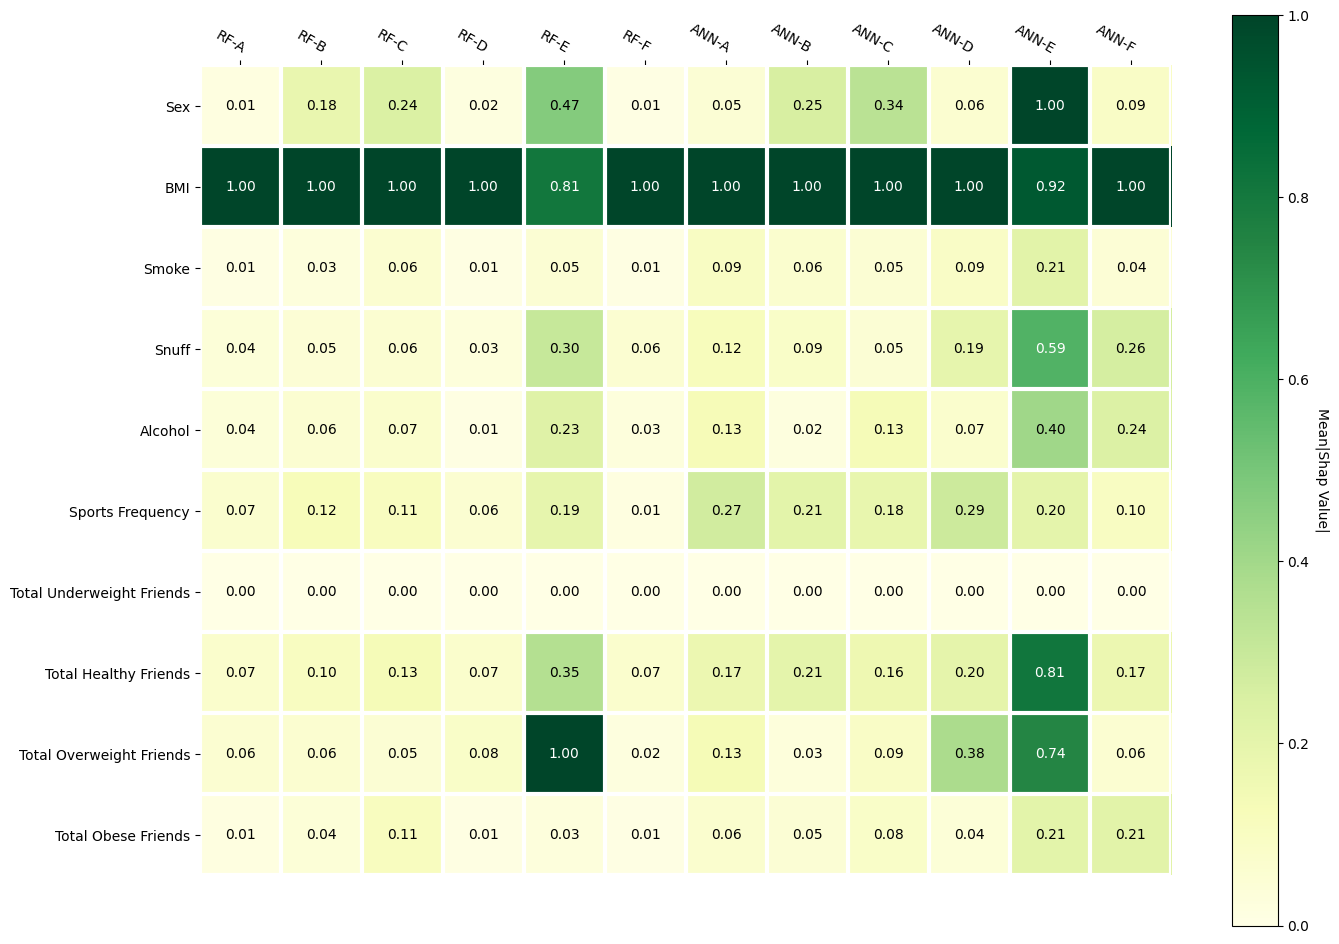
\includegraphics[width=0.9\linewidth]{figures/Results/ResultThree/Heatmap2.png } 
        \caption{Heatmap with the normalized mean |SHAP values| for the model with respect to each dataset (top names) against each variable (left names). Values closer to 1 indicate strong importance in the model.}
        \label{figure:Results3A}
    \end{figure}

    \begin{figure}[ht]
        \centering
            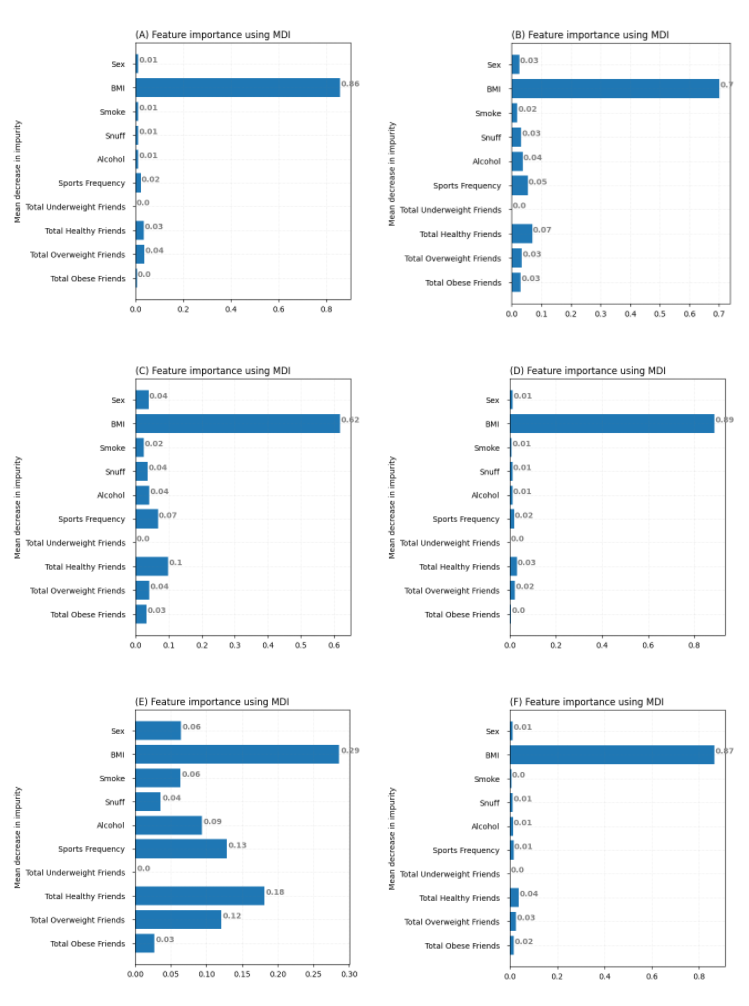
\includegraphics[width=0.9\linewidth]{figures/Results/ResultThree/MDIs.png } 
        \caption{Barplots using MDI in RF for each of the datasets. The x-axis represents the MDI value, the greater the value the greater the importance. The y-axis represents each of the studied variables.}
        \label{figure:Results3B}
    \end{figure}

It is possible to evaluate specific individuals to check what makes them gain or lose BMI in FF2 with respect to FF1. Here we present two examples using RF in dataset A (figures \ref{figure:ResultsSHAP1} and  \ref{figure:ResultsSHAP2}). Individual cases should not be extrapolated as variable weights for the whole dataset. 

    \begin{figure}[ht]
        \centering
            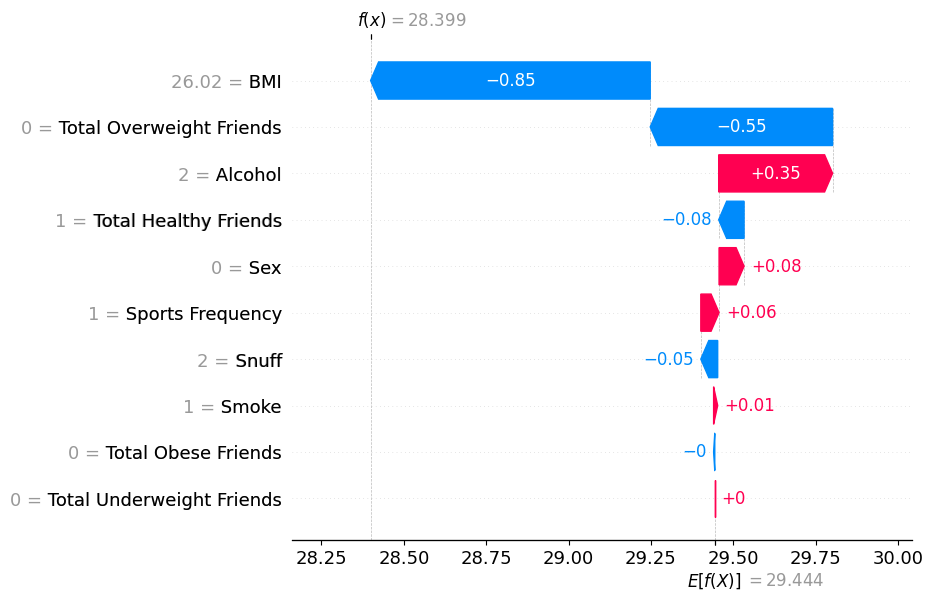
\includegraphics[width=0.9\linewidth]{figures/Results/ResultThree/Person Model RFA.png } 
        \caption{Waterfall plot with an individual case in the (A) dataset. The first row is the initial BMI in FF1, which was 26.09 (overweight) but is relatively close to 25 and this person is almost classified as healthy. This contributed the most (-0.85) to the final BMI in FF2 displayed on the figure’s top “f(x) = 28.399”, which increases below average in comparison with the rest of the samples in this dataset; with the average being 29.444 displayed on the bottom of the figure as “E[f(X)] = 29.2444”. After that, we see that having 0 overweight friends also contributed (-0.55) in favor of lowering the final BMI. The alcohol consumption of 2, equivalent to “Twice or more per month”, contributed in the opposite direction, increasing the final BMI to +0.35. One healthy friend contributed a little bit to decrease the final BMI. Being a man (sex = 0) contributed a little bit to worse BMI. And so on for the rest of the variables until the change becomes inconsequential. }
        \label{figure:ResultsSHAP1}
    \end{figure}

    \begin{figure}[ht]
        \centering
            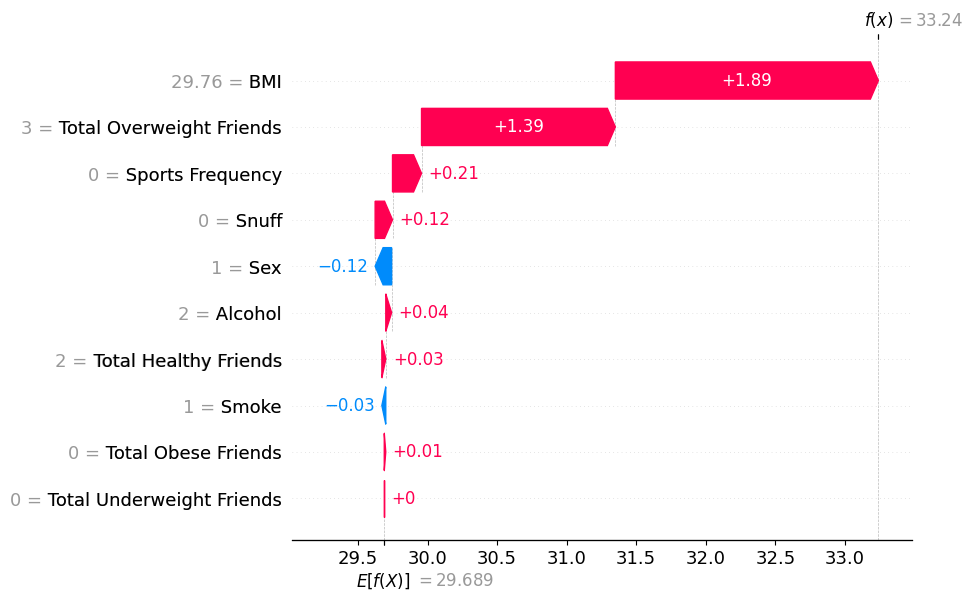
\includegraphics[width=0.9\linewidth]{figures/Results/ResultThree/Person ModelRFA 36.png} 
        \caption{Waterfall plot with an individual case in the (A) dataset. The initial BMI in FF1 was 29.68, very close to the obese category, which contributed the most to increasing the final FF2 BMI to 33.24, displayed in “f(x) = 33.24” at the top of the figure, by quite a lot (+1.89), in comparison with the FF2 average displayed at the bottom of the figure as “E[f(x)] = 29.689”. Having 3 overweight friends also contributed to a similar increase of +1.39. Not practicing any sport also contributed to a moderate increase in BMI (+0.21). The rest of the variables' effects’ sizes are quite small in comparison to the effects of the first three. }
        \label{figure:ResultsSHAP2}
    \end{figure}

Partial dependencies plots indicate how changing a particular variable changes the output of the model. All plots produced in this section are done using the RF models.

All datasets except C (Healthy to Healthy) show a decrease in BMI with respect to the total number of healthy friends (figure \ref{figure:Results3PDHealthy}). Datasets B (Overweight or Obese to better) and C also show a slight increase in BMI with sports, this might be due to an increase in muscle mass and reduced total percentage of fat due to exercise. Increasing the BMI is not necessarily bad if the increase is due to a higher weight due to increased muscle mass. So, in the C dataset, this increase seems to be justified due to staying healthy. In the B dataset, it would indicate that sports also help by decreasing total body fat. 

    \begin{figure}[ht]
        \centering
            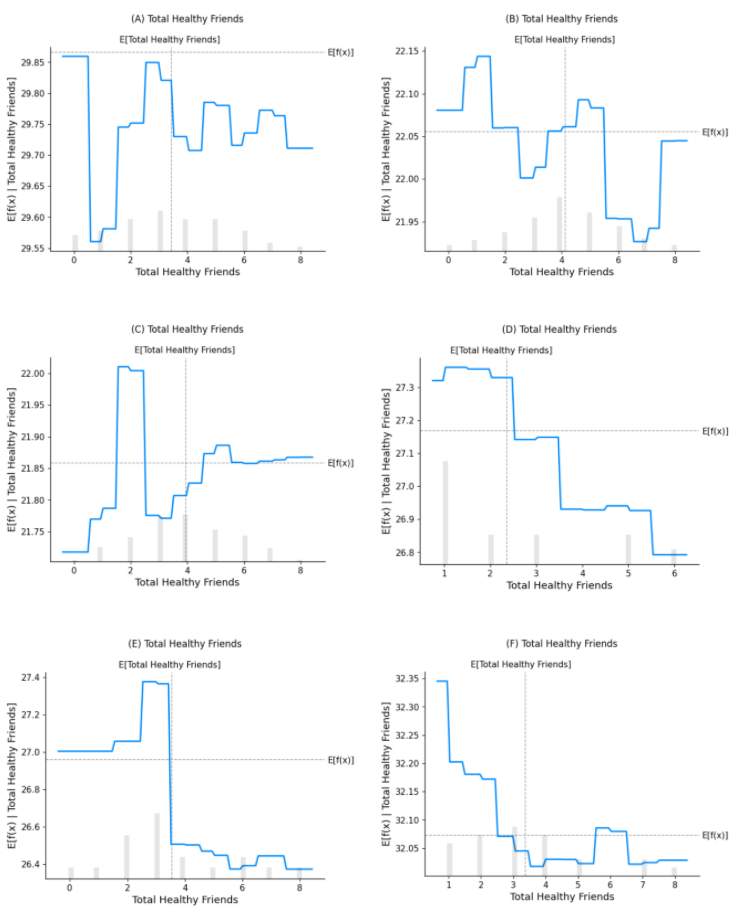
\includegraphics[width=0.9\linewidth]{figures/Results/ResultThree/PDHealthy.png } 
        \caption{Partial dependencies plots for datasets A to F in regard to total healthy friends for the RF models. On the X-axis, the total number of healthy friends, with a light grey histogram in the background. On the Y-axis, this variable is expected to modify the model output (BMI) as the variable changes.}
        \label{figure:Results3PDHealthy}
    \end{figure}

All datasets except for D (Overweight or worse got better BMI) showed an increase in BMI with respect to the total number of overweight friends (figure \ref{figure:Results3PDObese}). 

    \begin{figure}[ht]
        \centering
            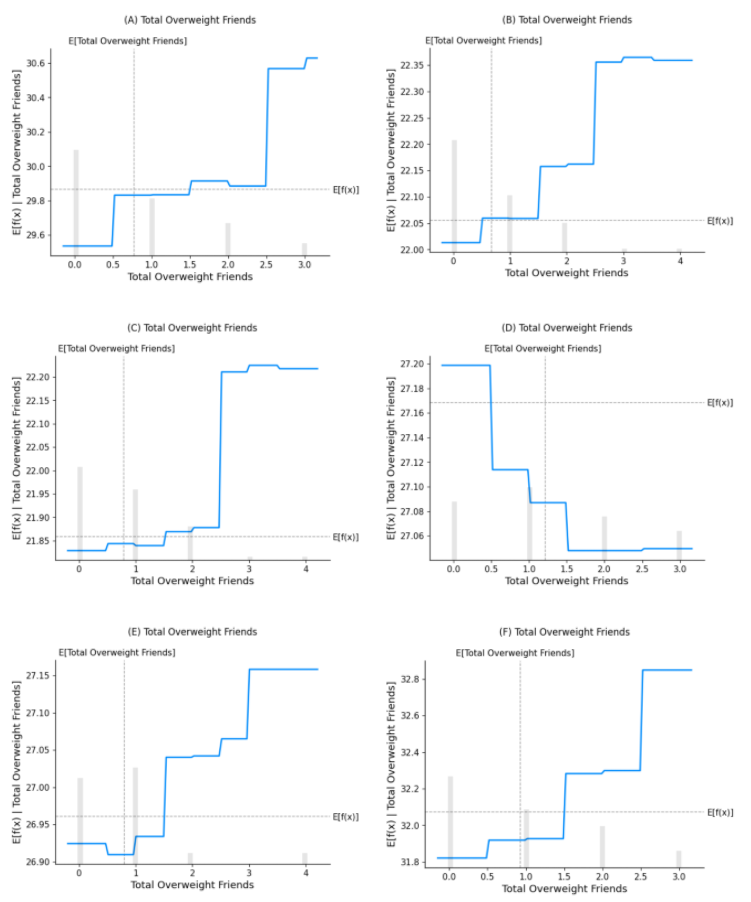
\includegraphics[width=0.9\linewidth]{figures/Results/ResultThree/PDOverweight.png } 
        \caption{Partial dependencies plots for datasets A to F in regard to total overweight friends for the RF models. On the X-axis, the total number of healthy friends, with a light grey histogram in the background. On the Y-axis, how this variable is expected to modify the model output (BMI) as the variable changes.}
        \label{figure:Results3PDObese}
    \end{figure}    

The dependency plots show on average a very slight increase (+0.12) in the final BMI. The weight of this variable is also low in the RF models. We show in the friendship bias section that obese individuals have low popularity and are not well connected with the healthy group. For all combined 692 valid samples, the average of total overweight friends is 0.28 ±0.56.  It would appear that increasing connectivity with obese individuals did not have a meaningful effect. However, since the connectivity is low, we can’t extrapolate on how the effect would be in a better-connected population. 
 
The E dataset (Healthy BMI that ends up in Overweight or worse) seems to have a completely different weight of SHAP values according to both RF and ANN (figure \ref{figure:Results3A}), and to MDI in RF (figure \ref{figure:Results3B}). Is also the group with the bigger BMI increase (+3.2 ±1.6). The variable Total Overweight friends get a very high impact on the model despite people not having that many overweight friends. In general, Total Healthy friends decrease the BMI but it shows a spike in BMI for specifically “3” healthy friends (figure \ref{figure:Results3PDHealthy}).  It shows an increase with smoke but a decrease with snuff and alcohol frequency (figure \ref{figure:Results3EWeird}). Females have slightly more risk than males. We tried limiting the dataset from Healthy to Overweight only in case the Healthy to Obese jump was too much of an outlier, but it had barely any effect on the outputs. Analyzing all individuals one by one using the waterfall plots did not show any pattern. Dataset C shows a spike in BMI for “2” total numbers of healthy friends (figure \ref{figure:Results3PDHealthy}), but the model is more predictable. E is just a subset of the A dataset which does not show any strange particularities either. 

    \begin{figure}[ht]
        \centering
            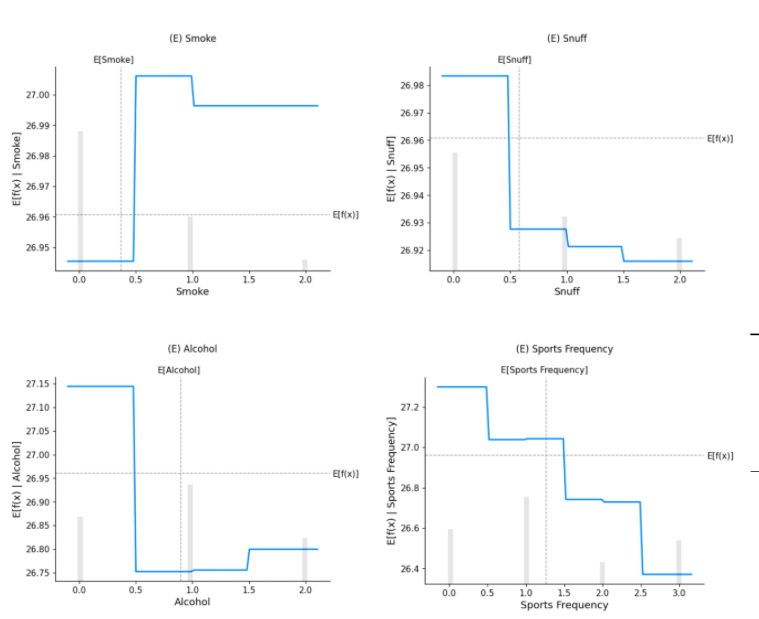
\includegraphics[width=0.7\linewidth]{figures/Results/ResultThree/PDECrap.png } 
        \caption{Partial dependencies plots for datasets E regarding recreational drugs and sport frequency for the RF models. On the X-axis, the total number of healthy friends, with a light grey histogram in the background. On the Y-axis, how this variable is expected to modify the model output (BMI) as the variable changes. }
        \label{figure:Results3EWeird}
    \end{figure}    

Similarly to Result I, here we evaluate the influence of friendship on obesity and it appears that there's also an influence depending on the number of "Healthy", "Overweight", or "Obese" friends. And our machine learning models give a similar explanation compared with previous results.

\clearpage



\section{Result IV}

\textbf{Frequency consumption of medication and social network influence in a general youth population.}

In previous studies there has been a concerning trend in self-medication and in particular the overuse of painkillers for non-therapeutic purposes; mostly as a recreational drug within Norway \cite{ref:selfMedicationA, ref:selfMedicationB, Lorentzen2018} which coincide with worldwide trends and usage \cite{Algarni2021, ijerph18115530, PolandSelfMedicate, Lein2023}. With this study, we aim for two objectives. First, to update the data on self-reporting medication with the FF1's 2010 data, and if possible, include up to Fit Futures 3 data done throughout the year 2022. And second to investigate if there's a social influence component as to whether students tend to self-medicate.

% and \ref{figure:Results4D}, unreferenced, taken away

We analyzed the frequency of self-reported consumption of medicines and diseases in our population (figure \ref{figure:Results4C}). We can observe that there are plenty of dermatological diseases, however, the usage of dermatological medicines is quite low. In contrast, the amount of pain-related diseases is low, but the consumption of painkillers, or anti-inflammatory medicaments is extremely high in comparison.

    \begin{figure}[H]
        \centering
            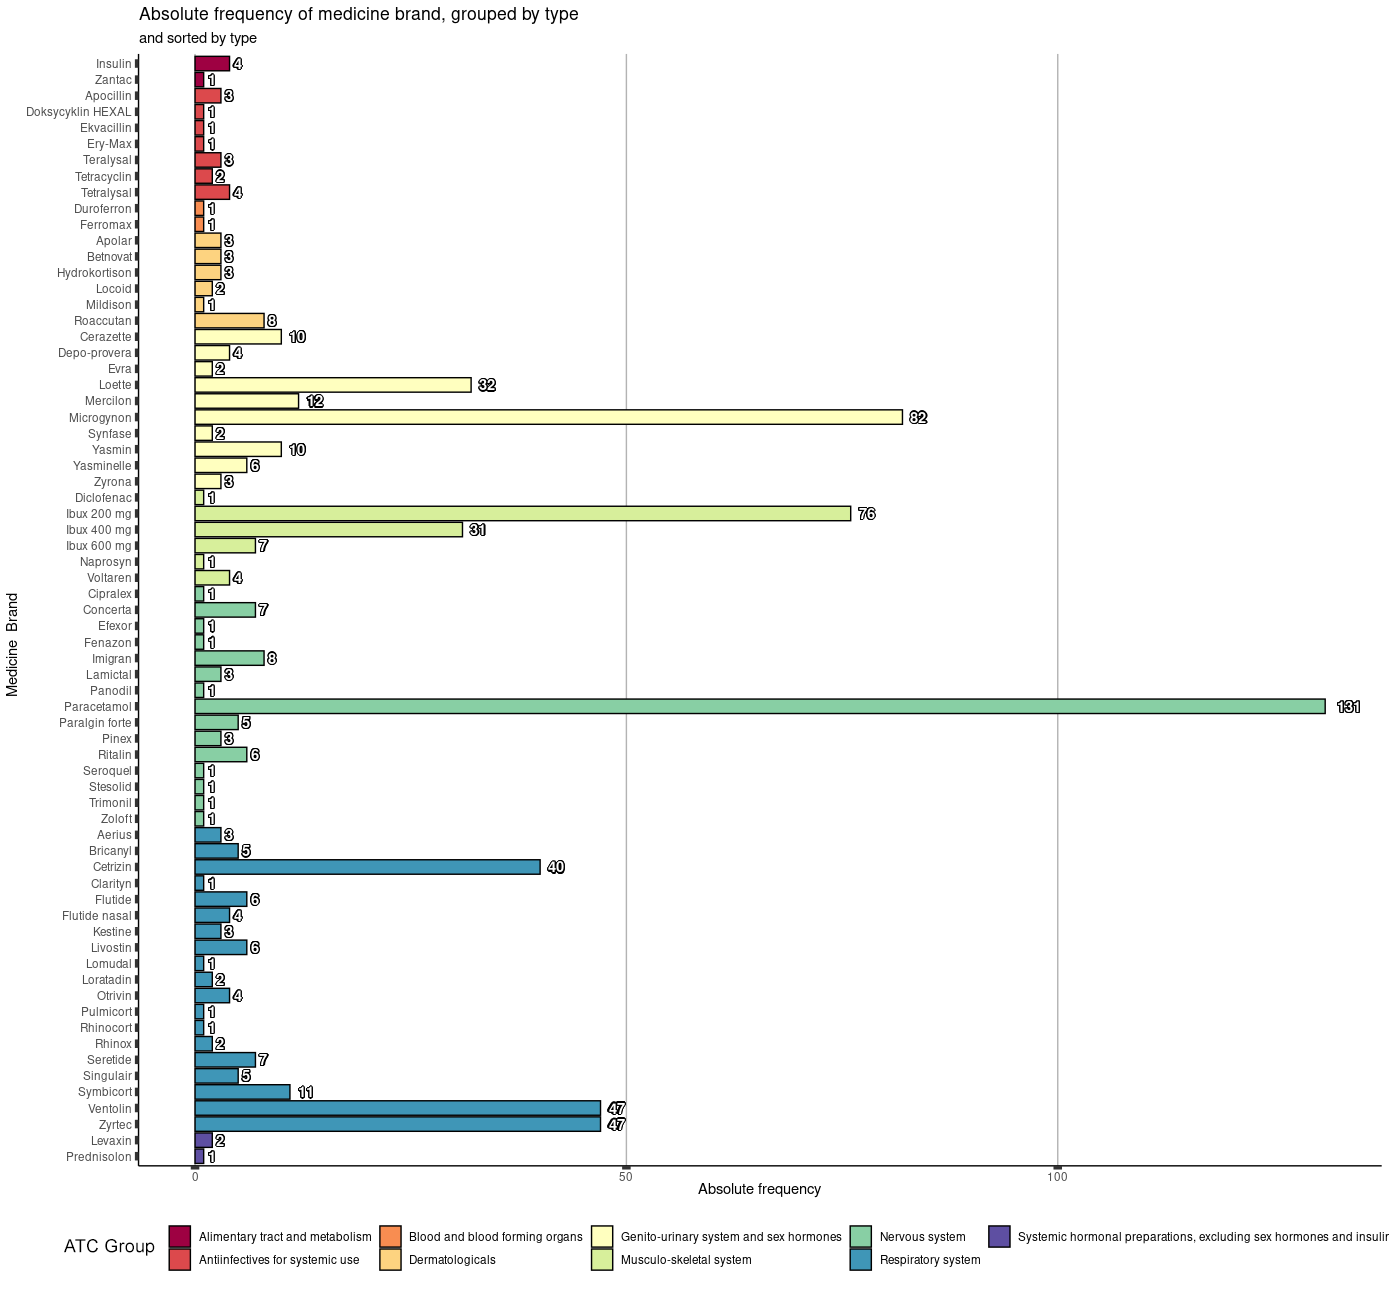
\includegraphics[width=0.9\linewidth]{figures/Results/ResultFour/CombinedLongRelBarPlot_typesAbsolute_Brand_TypeType.png } 
        \caption{Absolute frequency of medicine consumption sorted by ATC group. Hormonal contraceptives, anti-inflammatories, painkillers, antiasthmatic, and antihistaminics dominate the frequency of use.}
        \label{figure:Results4C}
    \end{figure}

Females seem to have a higher consumption of medicines in general (figure \ref{figure:Results4B}), and also higher disease prevalence (figure \ref{figure:Results4Diseases}). However, the disease types and medicine types don't match; meaning that self-medication is higher among the female population.

    \begin{figure}[H]
        \centering
            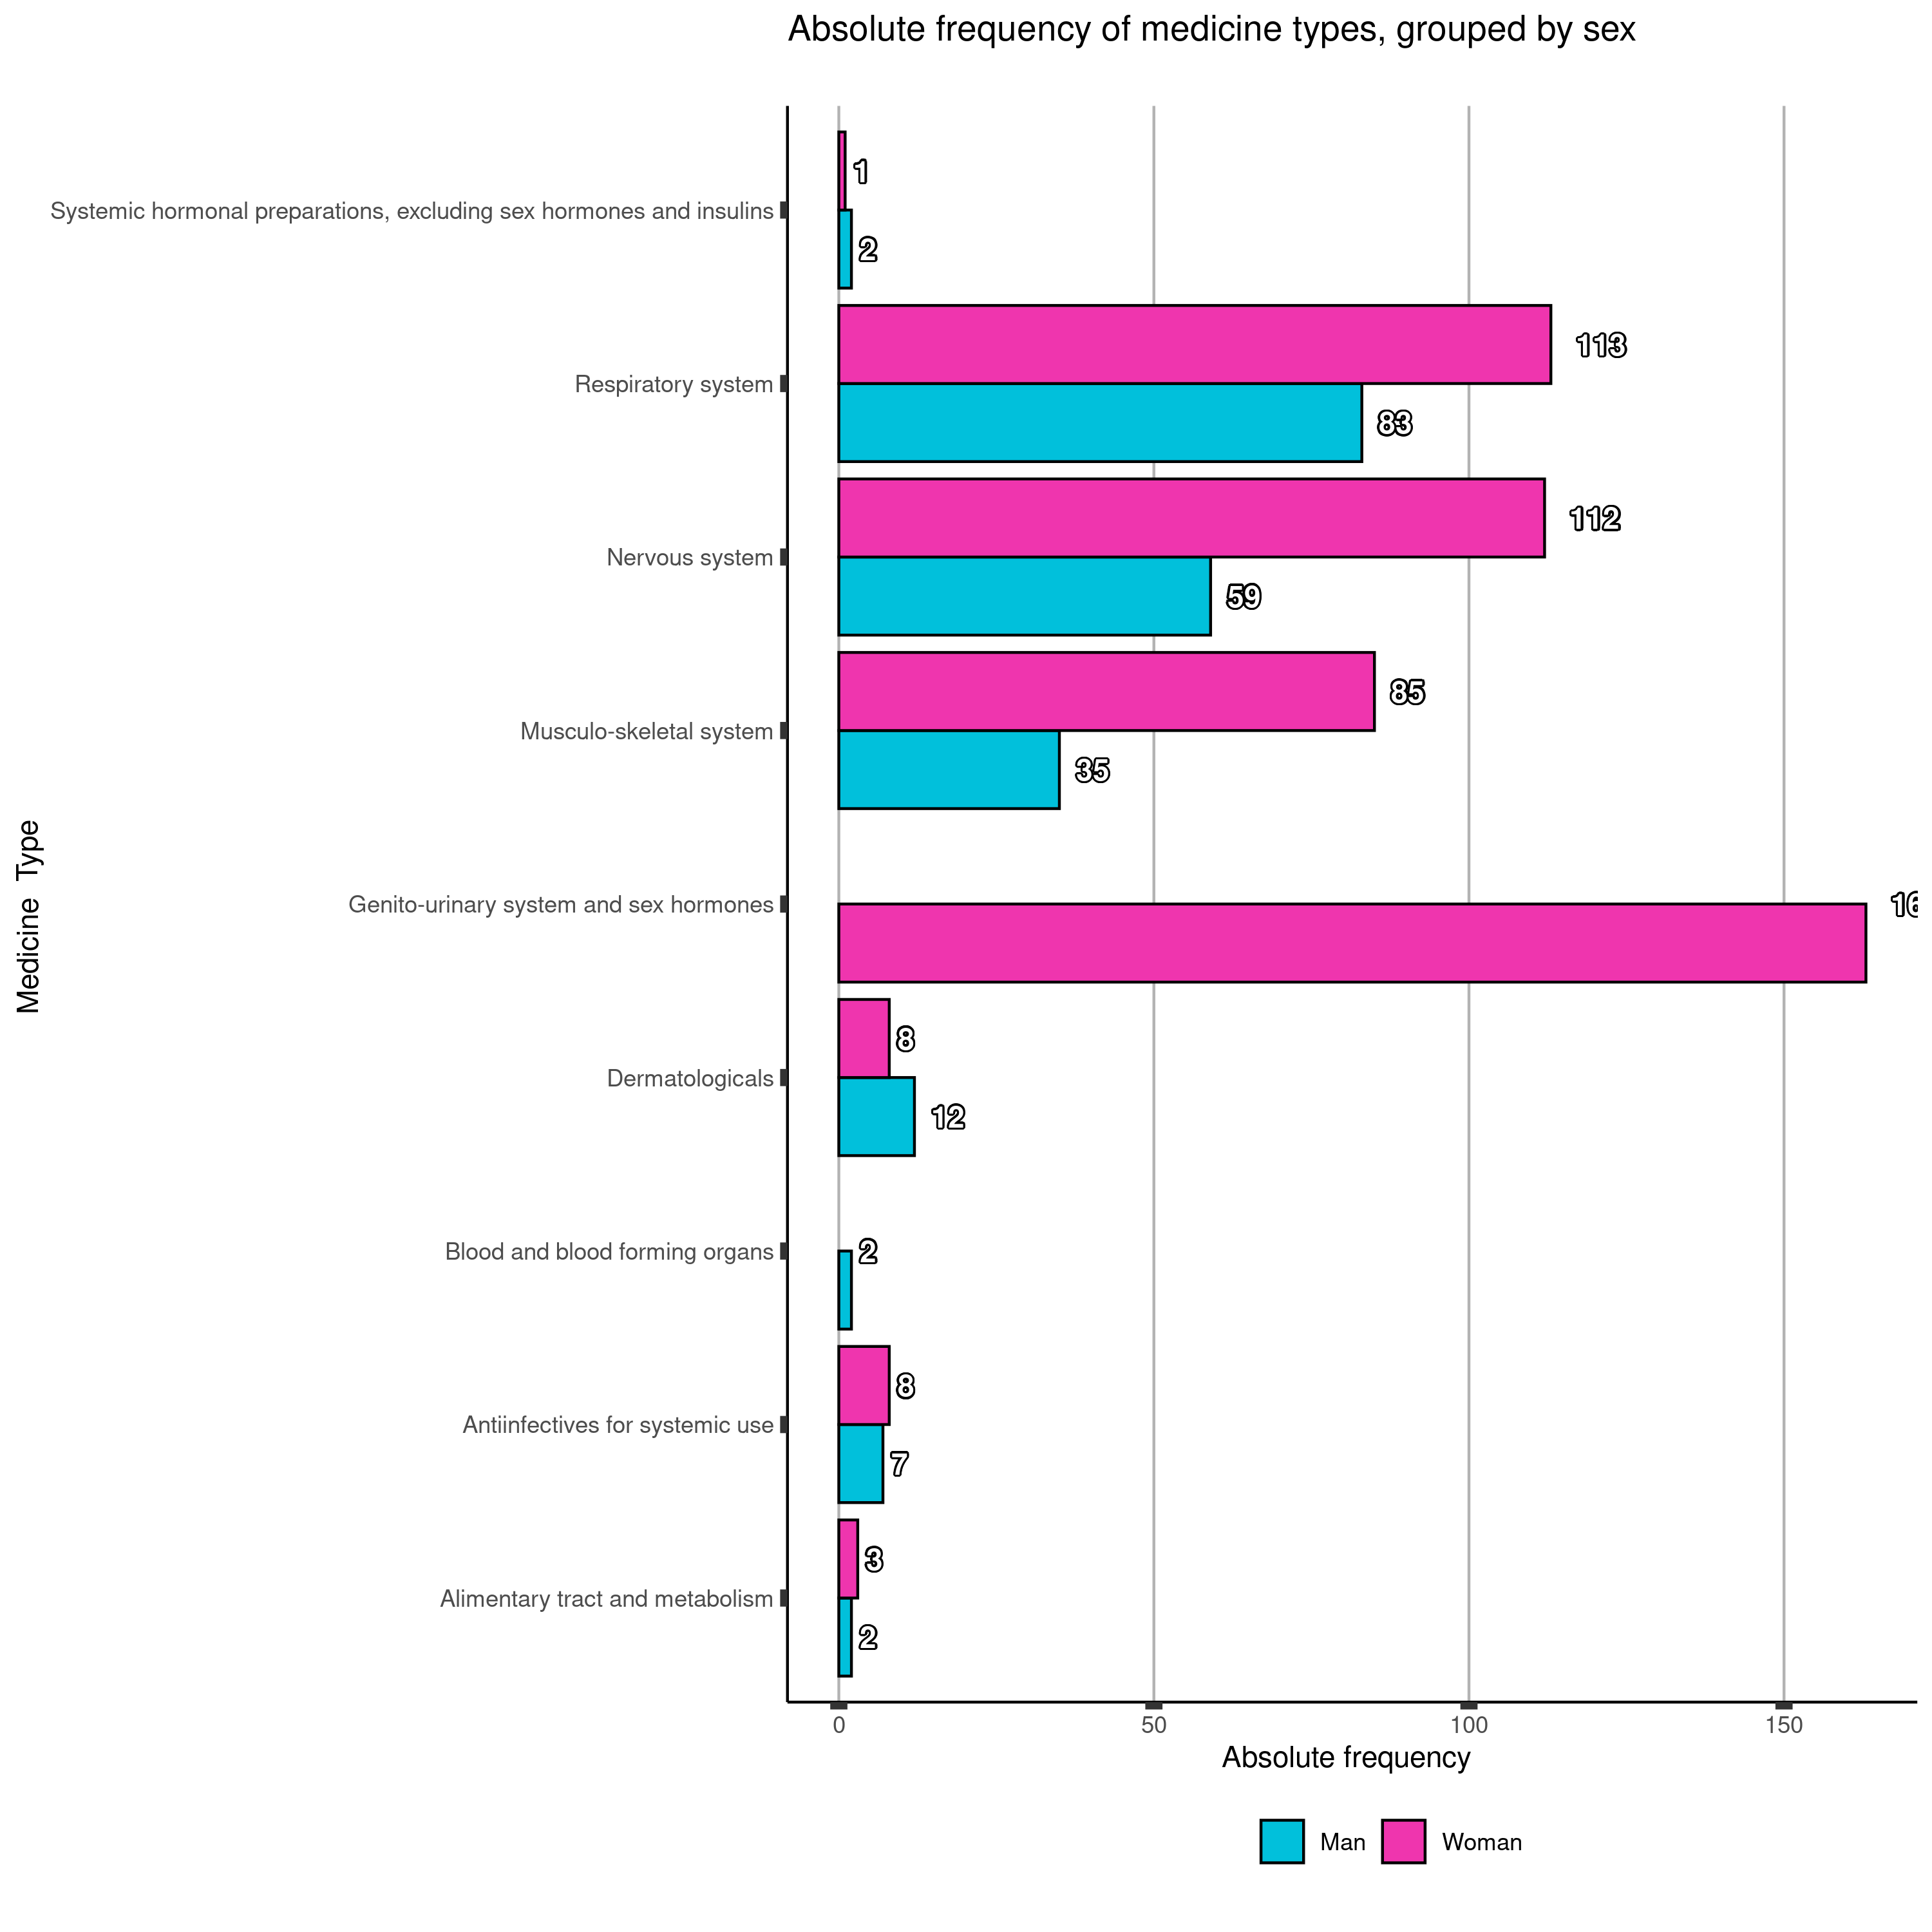
\includegraphics[width=0.9\linewidth]{figures/Results/ResultFour/CombinedLongAbsBarPlot_typesBySex_Type_Sex.png } 
        \caption{Absolute frequency of medicine consumption group by ATC group and divided by sex, which seems to indicate a higher consumption among females}
        \label{figure:Results4Diseases}
    \end{figure}

    
    \begin{table}
    
        \caption{Summary of the $Xi^2$ significance for relevant medicine groups divided by bias type (high school and sex). From left to right, bias type, type of medicine, numerical significance rounded to 4 decimals, and p-value in GP Prism 5.04/d format. Hormonal contraceptives seem to be biased concerning high school. Painkillers also seem to be biased by high school and sex. Anti-inflammatory shows a bias by sex only}
        
        \centering
        
        \begin{tabular}{clll}
        
            \rowcolor[rgb]{1,1,0.78} \multicolumn{1}{l}{Bias type}       & Medicine                             & Significance &       \\ 
            \hline
            {\cellcolor[rgb]{1,0.808,0.576}}                             & Hormonal contraceptives (women only) & 0.0002       & ***   \\
            {\cellcolor[rgb]{1,0.808,0.576}}                             & Anti-inflammatory                    & 0.2075       & ns    \\
            {\cellcolor[rgb]{1,0.808,0.576}}                             & Antihistamine                        & 0.1766       & ns    \\
            \multirow{-4}{*}{{\cellcolor[rgb]{1,0.808,0.576}}Highschool} & Painkiller                           & 0.0006       & ***   \\ 
            \hline
            {\cellcolor[rgb]{0.925,0.957,1}}                             & Anti-inflammatory                    & 0            & ****  \\
            {\cellcolor[rgb]{0.925,0.957,1}}                             & Antihistamine                        & 0.264        & ns    \\
            \multirow{-3}{*}{{\cellcolor[rgb]{0.925,0.957,1}}Sex}        & Painkiller                           & 0.0011       & **   
            
        \end{tabular}
        
        \label{table:Results4XiSummary}
        
    \end{table}

    \begin{figure}[H]
        \centering
            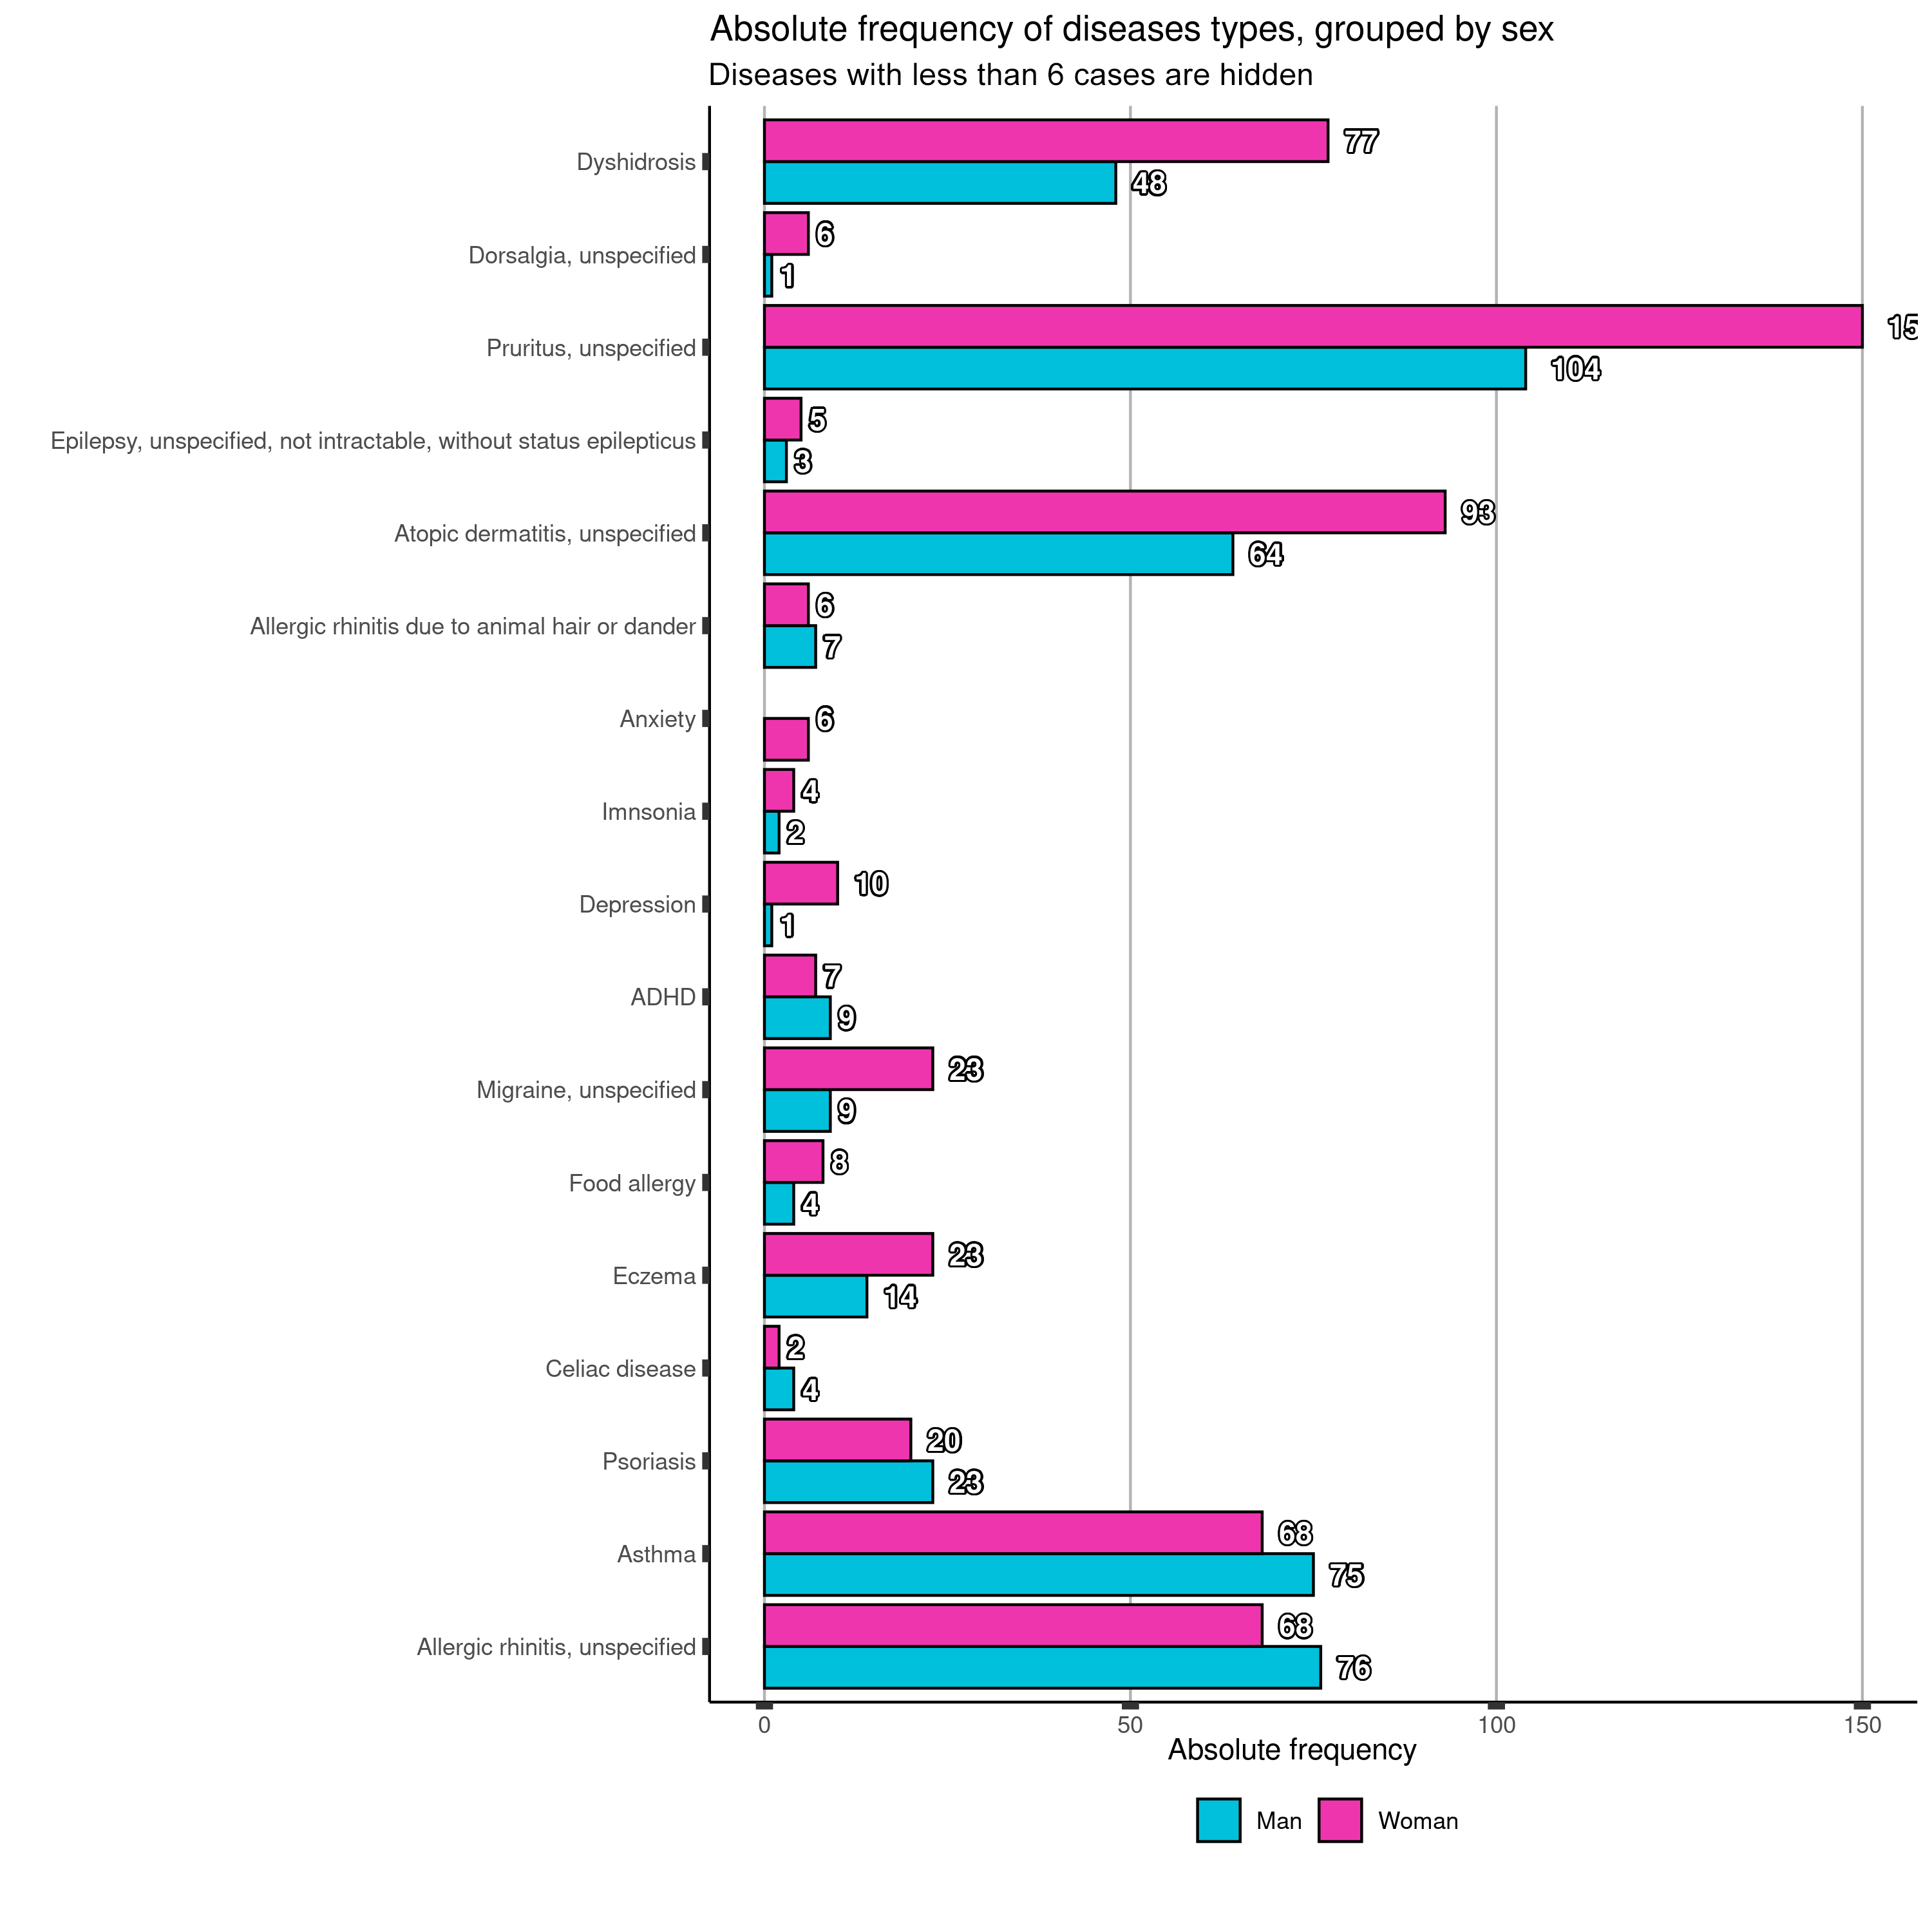
\includegraphics[width=0.9\linewidth]{figures/Results/ResultFour/CombinedLongAbsBarPlot_typesDiseasesBySex_Diagnostic_Sex.png } 
        \caption{Absolute frequency of self-reported diseases divided by sex. To avoid visual cluttering, diseases with 5 or fewer instances are not included in this figure. Females also lead in dermatological and psychological conditions, plus migraines. Males seem to have a short lead in respiratory conditions.}
        \label{figure:Results4B}
    \end{figure}

    %\begin{figure}[H]
     %   \centering
      %      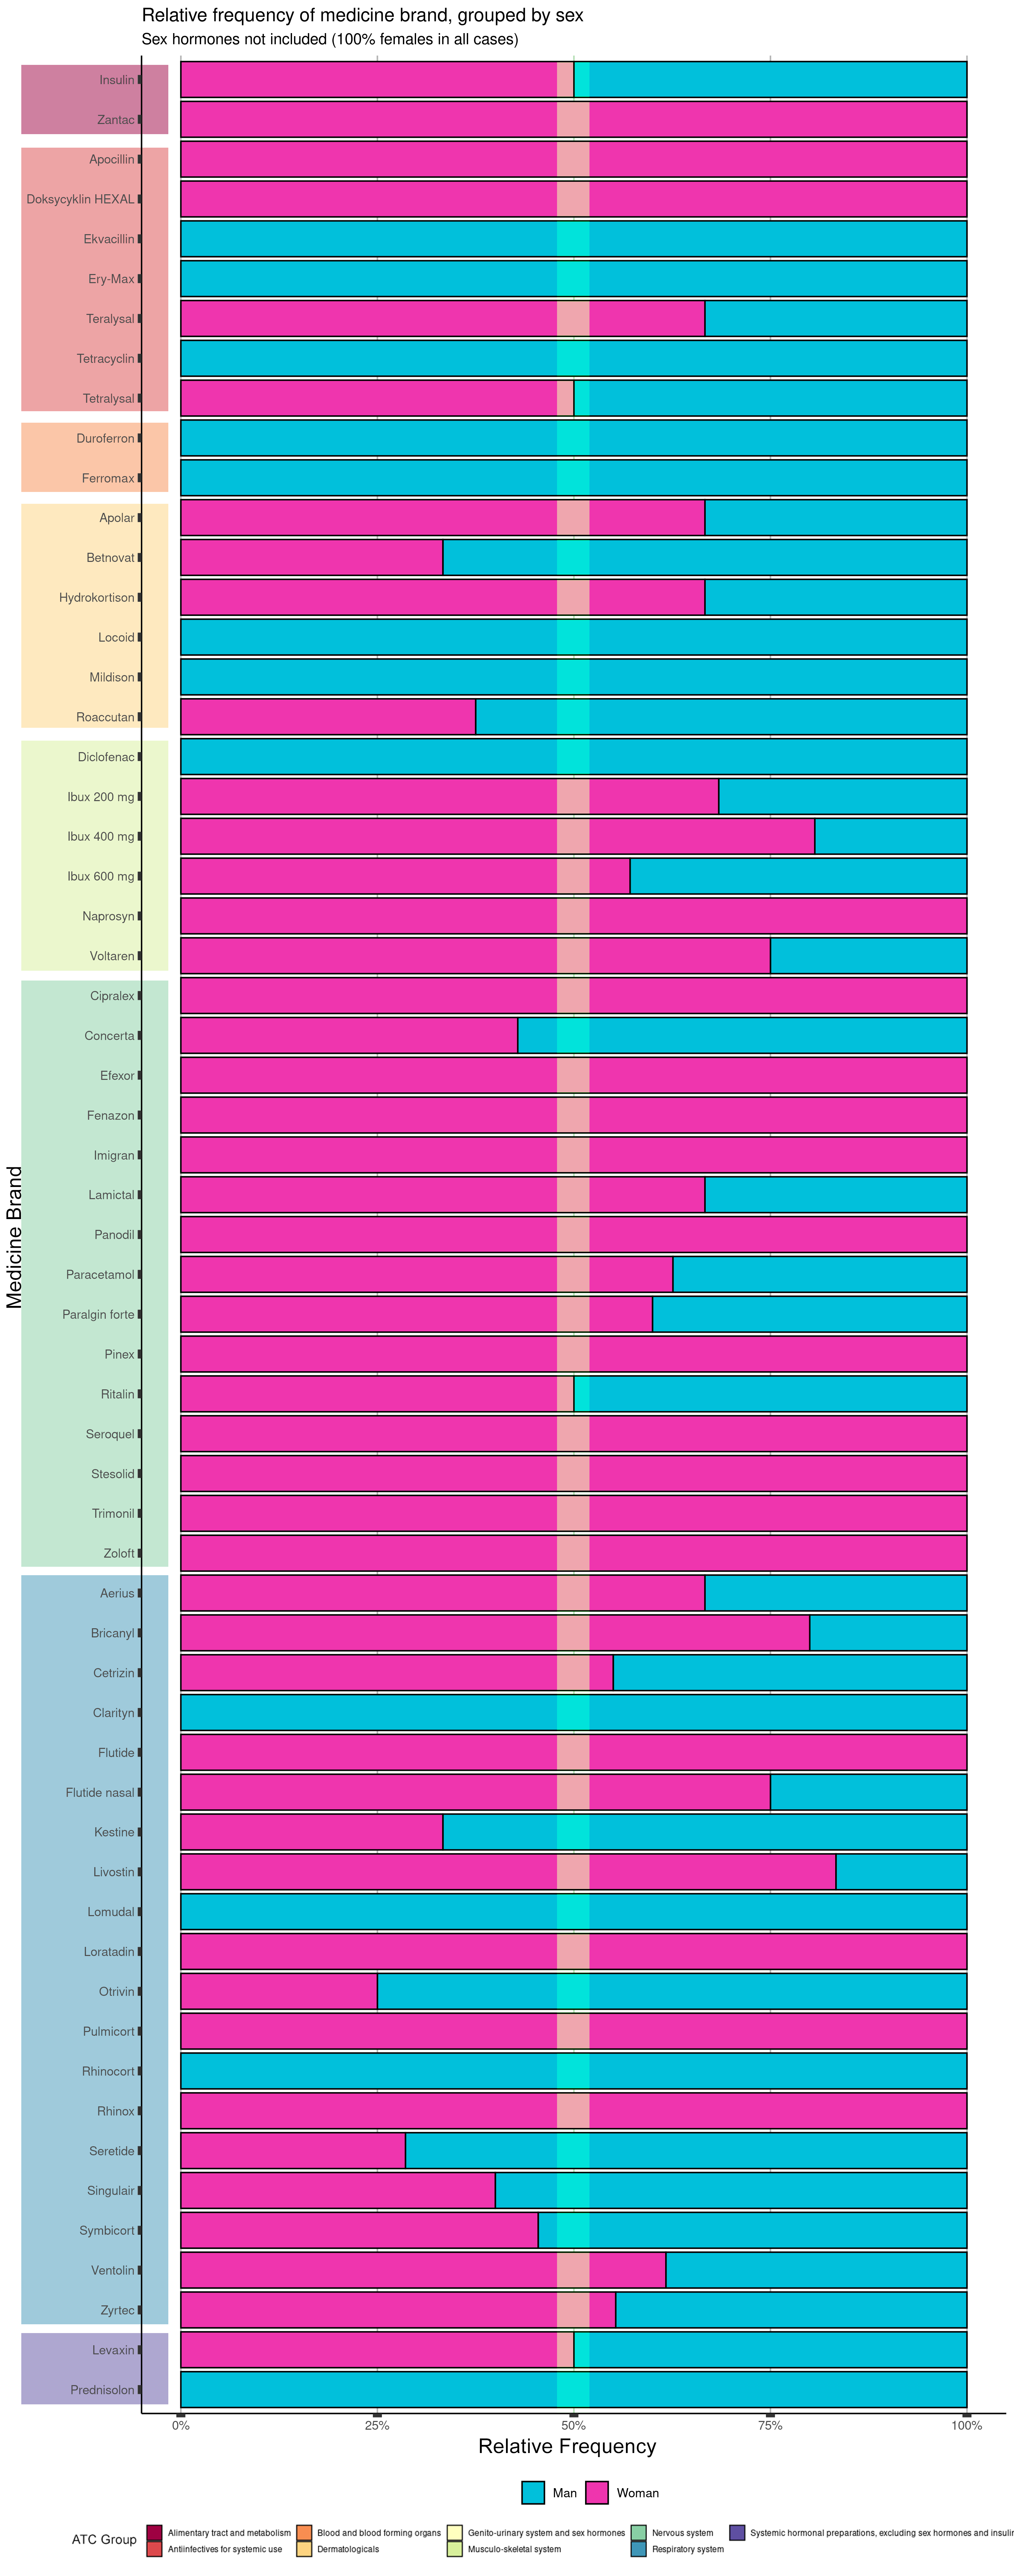
\includegraphics[width=0.5\linewidth]{figures/Results/ResultFour/CombinedLongRelBarPlot_typesBySex_Brand_Sex2.png } 
       % \caption{Relative consumption of medicines grouped by brand and divided by sex. Hormonal contraceptives are not included in the figure (100\% female). A highlight of ±5\% centered in the middle is included. Women seem to have a higher reported consumption of the most popular medicament.}
        %\label{figure:Results4D}
    %\end{figure}

We analyzed if there was any bias concerning sex and high school using over-the-counter medicines and also concerning hormonal contraceptives in women. Our results (table \ref{table:Results4XiSummary}) indicate that women sharing the same high school is biased towards hormonal contraceptive usage. Our simulations also show that women who are friends are biased to share the same hormonal contraceptive brand. One of the possible reasons is due to direct recommendations among them and later on asking their family doctor for the same brand. Another one is that women going to the same school tend to live close by and thus share the same family doctor who tends to prescribe the same medication.



The results coincide with teenagers' trend of misusing over-the-counter medication.
